\documentclass[conference]{IEEEtran}
\IEEEoverridecommandlockouts
% The preceding line is only needed to identify funding in the first footnote. If that is unneeded, please comment it out.
\usepackage{cite}
\usepackage{amsmath,amssymb,amsfonts}
\usepackage{algorithmic}
\usepackage{graphicx}
\usepackage{textcomp}
\usepackage{xcolor}
\usepackage{hhline}
\def\BibTeX{{\rm B\kern-.05em{\sc i\kern-.025em b}\kern-.08em
		T\kern-.1667em\lower.7ex\hbox{E}\kern-.125emX}}
\begin{document}
	
	\title{Adaptive-Precision Analog-to-Digital Conversion for Energy-Efficient Edge Intelligence\\}
	%An Efficient and Implementation-friendly Method of Precision-adaptive Column-parallel ADC Design for More Intelligent Edge Computing
	\iffalse
	\author{\IEEEauthorblockN{1\textsuperscript{st} Given Name Surname}
		\IEEEauthorblockA{\textit{dept. name of organization (of Aff.)} \\
			\textit{name of organization (of Aff.)}\\
			City, Country \\
			email address or ORCID}
		\and
		\IEEEauthorblockN{2\textsuperscript{nd} Given Name Surname}
		\IEEEauthorblockA{\textit{dept. name of organization (of Aff.)} \\
			\textit{name of organization (of Aff.)}\\
			City, Country \\
			email address or ORCID}
		\and
		\IEEEauthorblockN{3\textsuperscript{rd} Given Name Surname}
		\IEEEauthorblockA{\textit{dept. name of organization (of Aff.)} \\
			\textit{name of organization (of Aff.)}\\
			City, Country \\
			email address or ORCID}
		\and
		\IEEEauthorblockN{4\textsuperscript{th} Given Name Surname}
		\IEEEauthorblockA{\textit{dept. name of organization (of Aff.)} \\
			\textit{name of organization (of Aff.)}\\
			City, Country \\
			email address or ORCID}
		\and
		\IEEEauthorblockN{5\textsuperscript{th} Given Name Surname}
		\IEEEauthorblockA{\textit{dept. name of organization (of Aff.)} \\
			\textit{name of organization (of Aff.)}\\
			City, Country \\
			email address or ORCID}
		\and
		\IEEEauthorblockN{6\textsuperscript{th} Given Name Surname}
		\IEEEauthorblockA{\textit{dept. name of organization (of Aff.)} \\
			\textit{name of organization (of Aff.)}\\
			City, Country \\
			email address or ORCID}
	}
    \fi
	
	\maketitle
	
	\begin{abstract}
	
Energy efficiency is the primary design constraint for deep-learning empowered edge intelligence. Sensory data such as visual and audio are known to be redundant in nature. Exploiting such redundancy through adaptive precision is a promising approach to minimizing energy costs. However, as the first line of data sensing, existing analog-to-digital converters (ADCs) are equipped with fixed-precision capabilities, preventing the adoption of energy-efficient adaptive data analysis pipeline. 
	
	This paper presents an adaptive-precision ADC architecture to enable energy-efficient adaptive data analysis pipeline for edge devices. The proposed design utilizes a fine-grain power gating strategy to enable efficient and easy-to-implement run-time data precision adaptation. The proposed method has been applied to widely used column-parallel ADCs, with two ADC design studies targeting data-intensive CMOS image processing. Experimental results demonstrate that the proposed method can reduce ADC energy consumption by approximately 50\% while minimizing control circuit requirements.
	
\end{abstract}

\begin{IEEEkeywords}
	
	ADC, adaptive-precision, energy efficiency, edge computing
	
\end{IEEEkeywords}

	\section{Introduction}

Battery powered Internet-of-Things (IoT) devices, such as wearables, have been playing an important role in people's daily lives.
In recent years, the adoption of deep learning algorithms on IoT devices are becoming increasingly prevalent to empower edge
intelligence, such as machine vision, speech recognition, and robotics applications. Content-rich deep models are data and energy 
intensive, limiting their applications in energy-constrained, battery-operated IoT devices. There is an urgent need to tackle the 
energy challenge to support and sustain the fast expansion of artificial intelligence of things.

It is a known fact that feature-rich content, such as video and voice, has high data redundancy. Leveraging such data redundancy
can potentially reduce the computation and energy cost. To this end, adaptive-precision computing strategies have recently been 
proposed to improve the system energy efficiency. Zhao {\it et al.} proposed a deep reinforcement learning based adaptive-resolution 
framework for multi-task video analytics~\cite{zhao_reinforcement-learning-based_2022}. Lubana and Dick presented Digital Foveation, an energy-aware machine vision framework processing images in multiple rounds with adaptive-resolution~\cite{lubana_digital_2018}. LiKamWa {\it et al.} dynamically optimized the camera clock frequency for trade off between the sensing quality and energy efficiency~\cite{likamwa_energy_2013}.
While the recently proposed adaptive-precision computing techniques can effectively reduce the computation cost, Analog-to-digital 
converters (ADCs), as the the first line of the edge analytics pipeline, are equipped with fixed data precision capabilities, and
dominate the energy consumption of the data sensing stage of edge computing. For instance, as demonstrated in the previous study, 
such fixed-precision ADC design may introduce significant energy overhead to data sensing and communication, accounting for 50\%-75\% of overall energy in the image sensers~\cite{choi_energyillumination-adaptive_2015,takayanagi_125-inch_2005,kitamura_33-megapixel_2012}, and 34\% 
of the total machine vision analytics pipeline with backend digital hardware acceleration~\cite{likamwa_redeye_2016}.

This work introduces adaptive-precision ADC architecture design to tackle the energy efficiency challenge of edge intelligence. 
The proposed design leverages a fine-grained power gating strategy to enable efficient and implementation-friendly run-time precision 
adaptation. The proposed method has been applied to widely used column-parallel ADCs, with two ADC design studies targeting 
data-intensive CMOS image processing. Experimental results demonstrate that the proposed method can reduce ADC power consumption 
by approximately 50\% with only a few required control circuits. This work makes the following contributions. 

%While more and more deep-learning algorithms have harnessed the redundancy of sensory data to improve the energy efficiency through precision-adaptive computing \cite{leibe_xnor-net_2016}\cite{li_ternary_2016}\cite{park_energy-efficient_2018}, 

%of edge devices, are still generally equipped with fixed precision capabilities. Therefore, opportunities have been offered for adaptive-precision tuning within the ADCs to further lower the energy barrier of edge sensing and computation. 
%and implementation with CIM architecture \cite{chiu_4-kb_2020}\cite{karunaratne_-memory_2020}\cite{jung_crossbar_2022} have been extensively studied, 
%can also be precision-adaptively designed for more intelligent edge computing.
%can also be smartly designed for more intelligent edge computing. 

%As the NN models have been able to process data of varying precision for efficient multi-task analysis [xxxx], opportunities have been offered for us to further improve 
%the systems' energy efficiency by taking algorithm-aware adjustments inside the ADCs. Considering the precision (i.e. the quantization bits) is at the heart of an ADC’s energy constraints, 
%making it dynamically adaptive will be promising.

\begin{enumerate}[\IEEEsetlabelwidth{3)}]
	\item 
	An adaptive-precision ADC architecture is proposed to enable energy-efficient adaptive data sensing and computing for edge devices. The proposed design leverages a fine-grained power gating strategy to enable efficient and implementation-friendly run-time precision adaptation.
	Several auxiliary circuits have been carefully inserted to eliminate potential metastability caused by power gating. And the additional control signals are reused as much as possible or even not required, achieving cost-effective power-scaling capability exploitation inherently for the proposed ADC architectures.
	\item 
	The proposed method has been applied to widely used column-parallel ADCs targeting data-intensive CMOS image processing~\cite{kim_11-bit_2021,nie_single_2020,kumagai_14-inch_2018,park_640_2020}, with two case study ADC designs, including 
	a column-parallel Single-Slope (SS) ADCs~\cite{snoeij_18v_2005,kleinfelder_10000_2001} and a column-parallel Successive Approximation Register (SAR)/SS ADCs~\cite{kim_area-efficient_2016}. 

%	Both of the two architectures are completely built with not only main functional modules but also peripheral circuits including bandgap circuits, bias circuits and necessary buffers. And the ADCs' energy distribution across different modules is analysed  in detail. 
	%Two case study ADC designs applied in the CISs are presented with different design specifications.
    %according to which a method combining adaptive precision and fine-grained power gating strategies is proposed
    %for more smart data conversion.   

	\item 
	Experimental results demonstrate that the proposed method can effectively reduce ADC power consumption by approximately 50\% with only a few required control circuits.

	%Although with different design specificaitons, the proposed method is successfully applied to the two ADC architectures with the same principles, which shows universalty. Besides, the strengths and weaknesses of the two diffenrent architectures are specifically discussed.
\end{enumerate} 

The remainder of this paper is organized as follows. 
Sect.~\ref{related} presents some related works.
Sect.~\ref{architecture} shows the architecture overview of the two case study ADC designs. 
Sect.~\ref{strategy} describes the implementation of the proposed method for the two case study ADC designs. 
Sect.~\ref{result} reports the eluavation results and Sect.~\ref{discussion} develops discussions. 
Finally, Sect.~\ref{conclusion} concludes this paper.

	\section{Related Works}\label{related}

There have also been some prior work on adaptive-precision ADC design~\cite{zhu_06_2013,zhu_6--10-bit_2015,el-halwagy_100-mss5-gss_2018}. 
\cite{zhu_06_2013} and \cite{zhu_6--10-bit_2015} focused on a SAR ADC with splittable capacitor array for 8-10-bit or 6-10 bit adaptive-precision. 
\cite{el-halwagy_100-mss5-gss_2018} presented a time-domain SAR/Flash ADC using voltage-controlled oscillators (VCOs). The ADC can be configured as a double sampling SAR ADC for the high-resolution modes or as a 4× asynchronous time-interleaved Flash ADCs for the high sampling rate modes.
However, it is a known fact that it is difficult to implement VCO-used ADCs in the narrow readout channel pitch of the CMOS Image Sensor (CIS) due to its high circuit complexity~\cite{kim_area-efficient_2016}. In addition, a SAR ADC also introduces large area overhead to implement the Capacitor Digital-to-Analog Converter (CDAC)~\cite{funatsu_62_2015}.
Different from the prior work, we consider column-parallel SS ADC, which has been widely used for image processing applications, 
thanks to its small area and high linearity~\cite{kim_11-bit_2021,nie_single_2020,kumagai_14-inch_2018,park_640_2020}. 
In addition, SAR/SS ADCs have been studied~\cite{kim_area-efficient_2016,chen_12_2014} for reducing the A/D conversion time of 
the SS ADC and the area of the SAR ADC.     
In this work, we focus on enabling adaptive-precision for the SS and SAR/SS ADCs. Thanks to the SS conversion logic, exponential power 
scaling capability can be achieved through fine-grained power gating strategies, which has hardly been exploited before.

%Other works have tried to relieve the design specifications of ADCs by applying low-precision analog computing firstly close to the sensor~\cite{chen_asp_2016,liu_ns-cim_2020}. But high-precision ADCs and DNN processors are still required for complex tasks. Therefore, adaptive-precision tuning within ADCs remains competitive for efficient hardware reuse.

The proposed work aims to enable energy-efficient edge intelligence.  Adaptive-precision deep learning algorithms have been intensively studied~\cite{leibe_xnor-net_2016,li_ternary_2016,park_energy-efficient_2018} to enable energy-efficient edge intelligence. These prior works often apply a precision lower bound to optimize energy efficiency while ensuring the necessary accuracy.  The proposed adaptive-precision ADC design needs to account for this accuracy requirement to enable a complete adaptive-precision data analytics pipeline.  In this work, taking such constraint into consideration, we choose 4-bit conversion as the low-precision mode of the ADC, which achieves a good compromise between energy efficiency and algorithm accuracy. 

%Although these works are about downstream low-precision algorithms and relatively separated from the ADCs, the adaptive-precision design of ADCs needs to take the accuracy requirements of the algorithms into consideration for the complete pipeline. In this paper, we choose 4-bit conversion for the low-precision mode of the ADCs, with a trade off between the energy-saving capabilities of ADCs and accuracy loss of algorithms.

%\cite{leibe_xnor-net_2016} introduced Binary Weight Nets (BWN) and XNOR-Nets to enable Deep Neural Networks (DNNs) with binary weights and activations.  With some accuracy compensation strategies, BWN and XNOR-Nets are able to perform low-precision computations with only 0.8\% and 11\% accuracy loss, respectively.  \cite{li_ternary_2016} adopted weights of three values (i.e., -w, 0, w) to further reduce the accuracy loss of computing. Although this requires an additional bit per weight compared to binary weights, the sparsity of the weights can be exploited to save computation and storage resources.  \cite{park_energy-efficient_2018} presented an outlier-aware accelerator performing dense and low-precision (4-bit) computations on most of the data, while efficiently handling a small number of sparse and high-precision outliers.  


	\section{Adaptive-precision ADC Design}\label{architecture}

This section presents the proposed adaptive-precision ADC design. Targeting image processing applications, we consider SS and SAR/SS ADCs, which are suitable for image sensor integration. 
Section~\ref{over1} and \ref{over2} provide architecture overview of SS and SAR/SS ADCs. 
Section~\ref{gating1} presents the proposed power gating method. 
Section~\ref{gating2} and \ref{gating3} present adaptive-precision tuning of SS and SAR/SS ADCs. The key characteristics of the proposed adaptive-precision ADC architecture are summarized 
as follows. 

%The basic modules of the two ADC designs is overviewed firstly in \ref{over1} and \ref{over2}. Then, after showing the power gating implementation in \ref{gating1}, the adaptive-precision tuning within SS and SAR/SS ADCs is specifically described in \ref{gating2} and \ref{gating3}, with the following architectural enhancements:

\begin{enumerate}[\IEEEsetlabelwidth{3)}]
	\item 
	The thermometer-code counter in SS ADC is extended to support high/low-precision modes for adaptive-precision conversion, which can also provide an exponentially long window of opportunity for power gating.
	\item
    Stability-optimizing switches are inserted into the comparators in SS ADC to avoid unpredictable latch for low-precision conversion due to comparator power off. 
    \item
    Additional control signals in SAR/SS ADC are carefully reused and effectively minimized, enabling efficient power-scaling capabilities with limited numbers of shared level-shifters and inverters.      
\end{enumerate} 


%For other ADCs of different architecture, the proposed method can also be adopted.

\subsection{SS ADC Architecture Overview}\label{over1}

The overall architecture of SS ADC is presented in Fig.~\ref{SSADC}. The main modules include column-parallel correlated double sampling (CDS) circuits, comparators, 
and a column-shared ramp generator. Fig.~\ref{SSWAVE} shows the operational waveform of SS ADC. When the ramp signal exceeds the output of the CDS circuit in a specific column, 
the corresponding comparator is flipped and latches the time information $\Delta t$ into the following 8-bit latch as the conversion results. 
Such conversions across all columns is done as soon as the ramp signal reaches $V_{refh}$.

\begin{figure}[htbp]
	\centerline{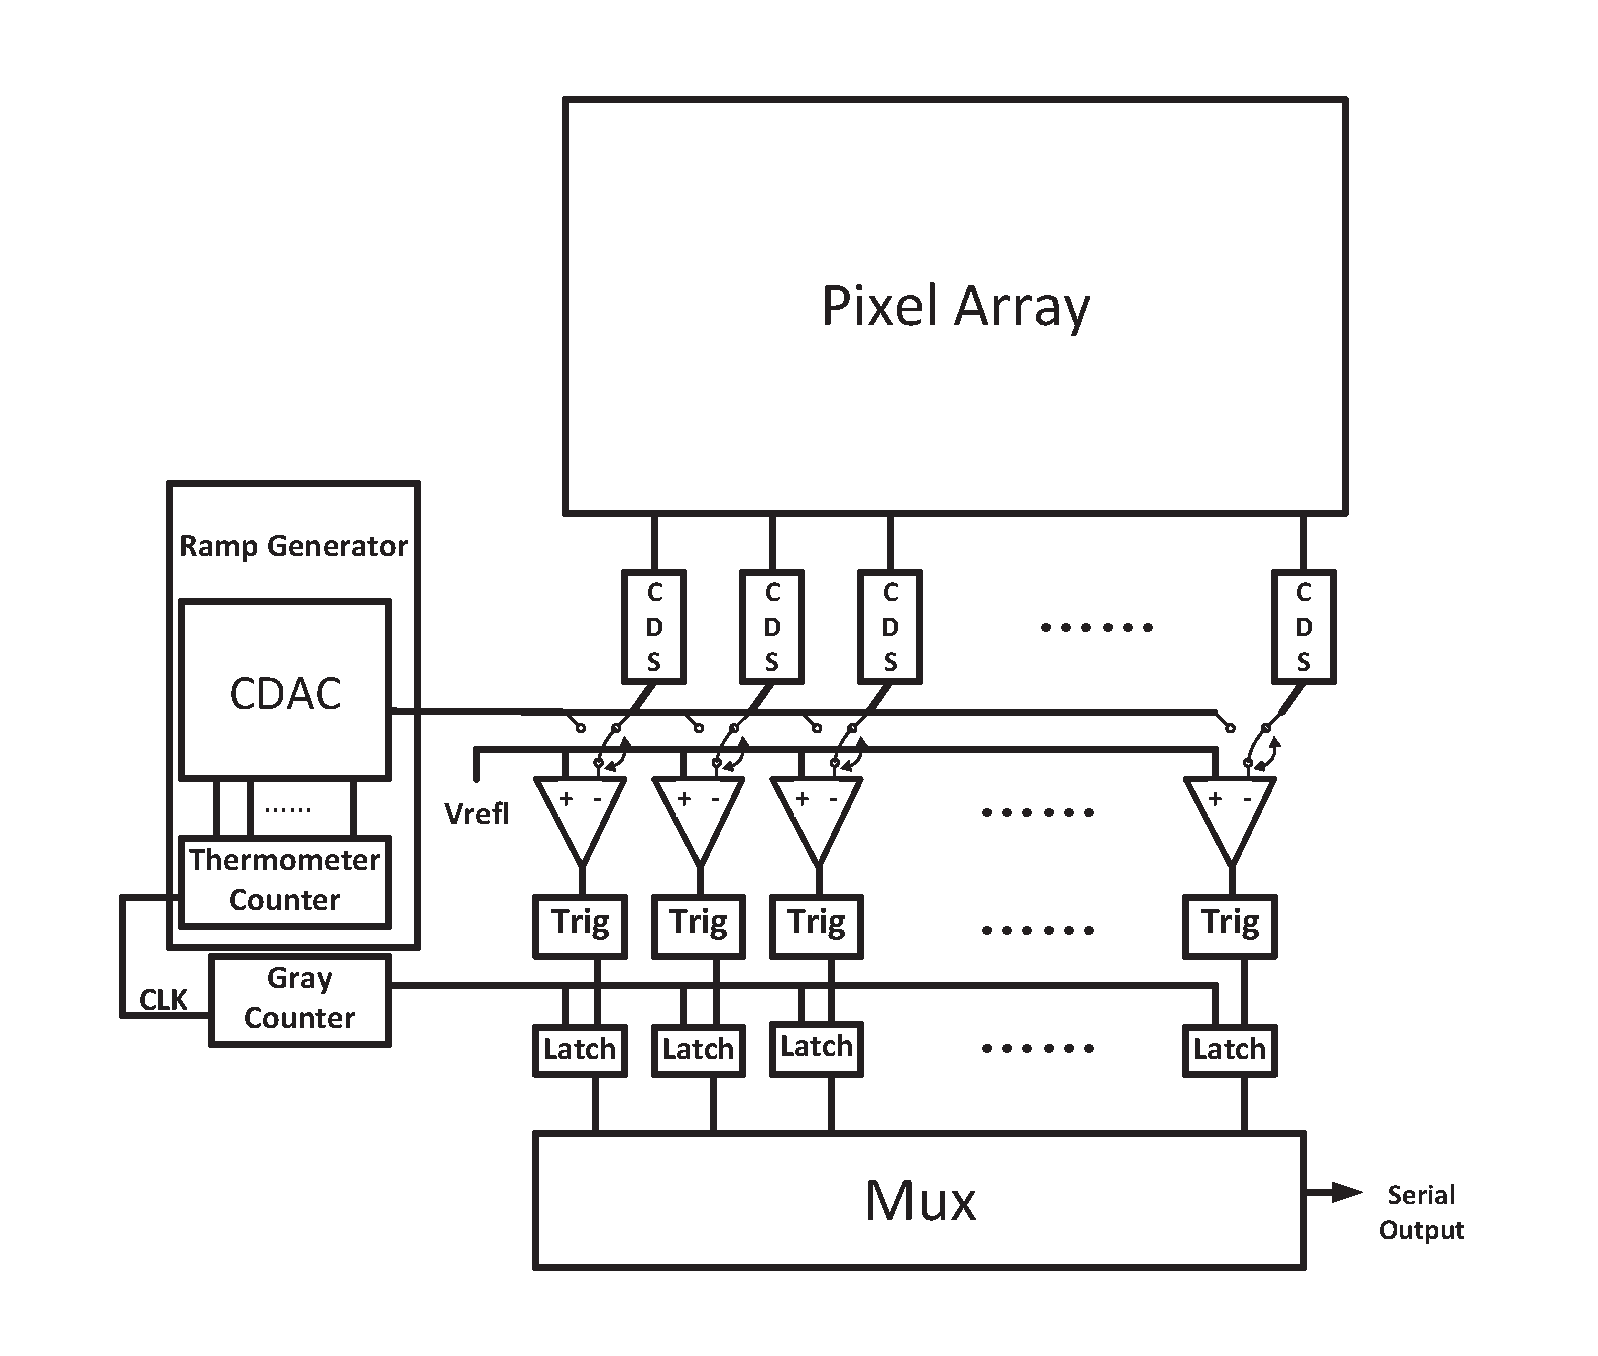
\includegraphics[width=3.5in]{./Figures/SSADC.eps}}
	\caption{The overall architecture of SS ADC.}
	\label{SSADC}
\end{figure} 

\begin{figure}[htbp]
	\centerline{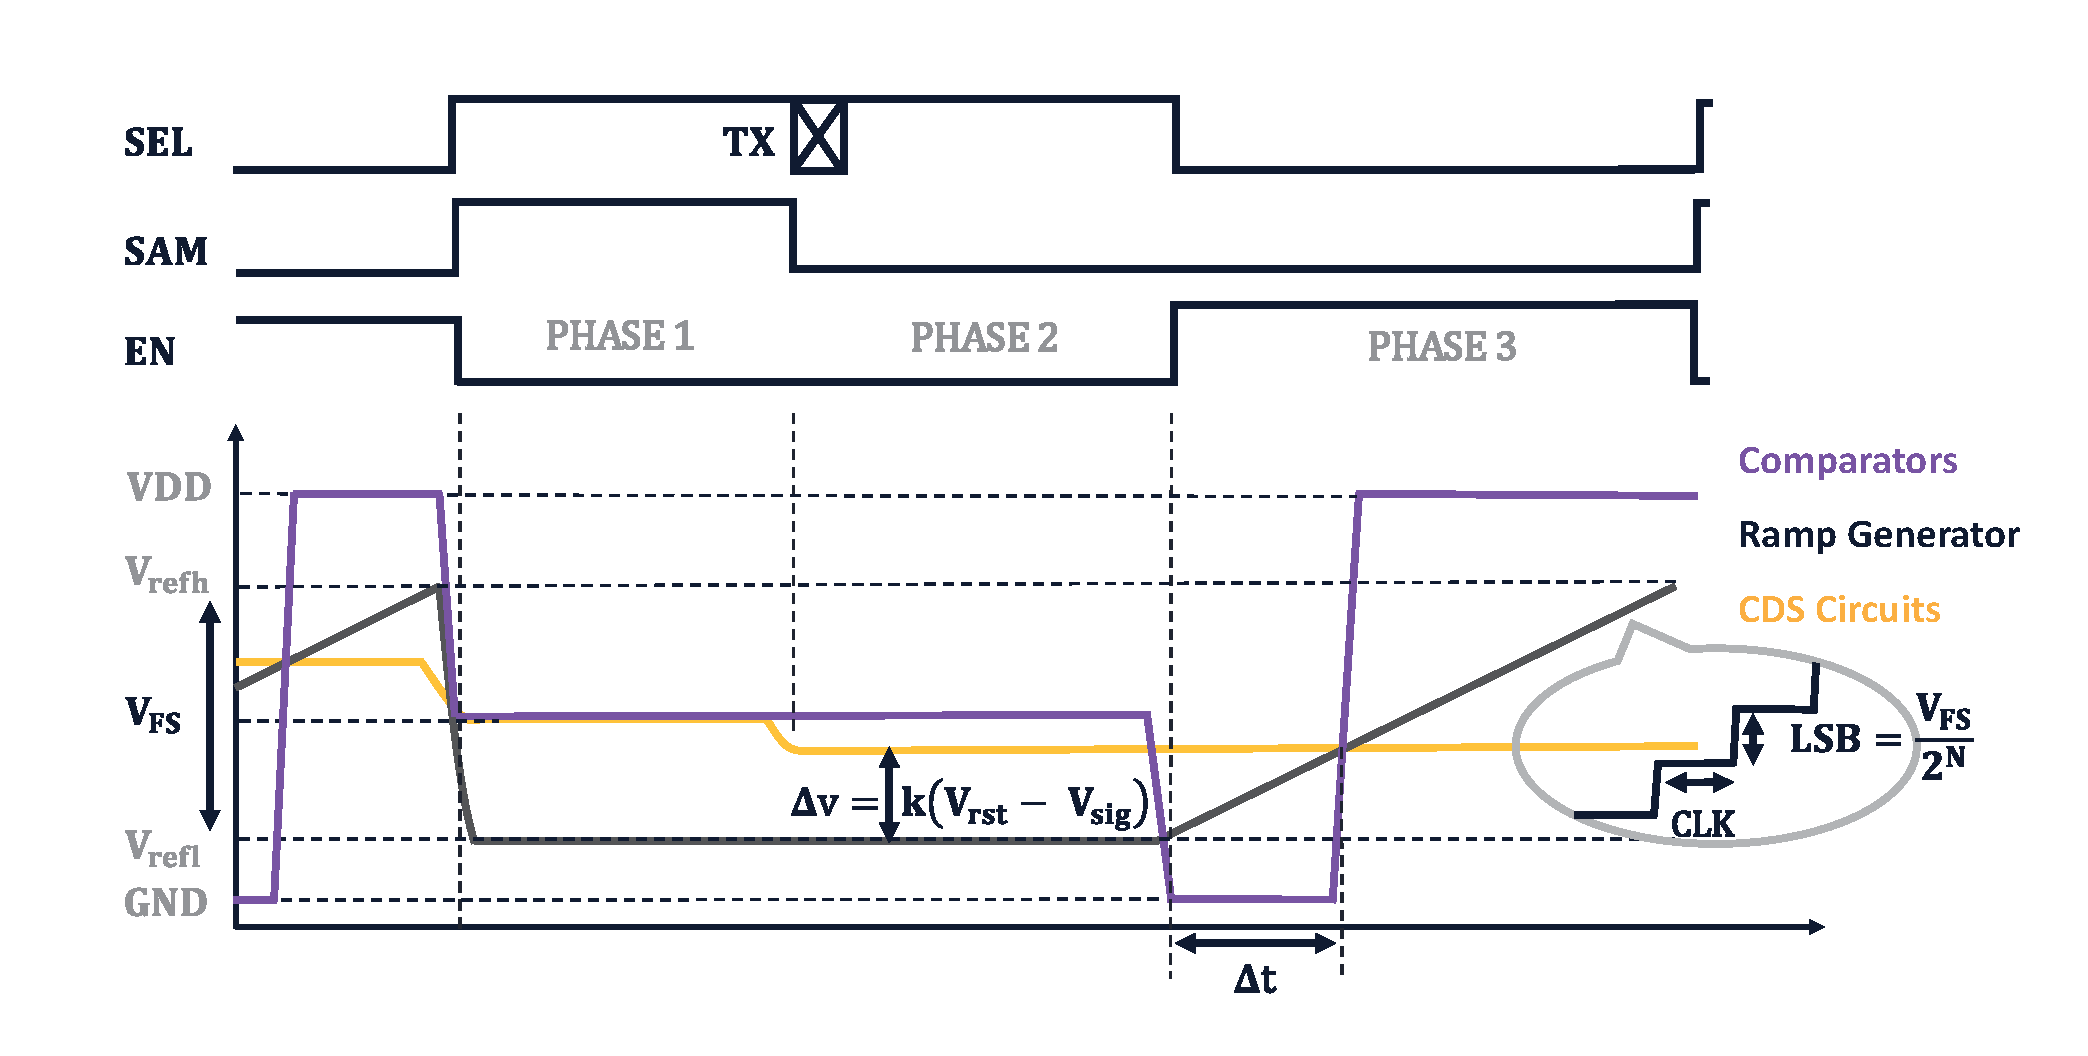
\includegraphics[width=3.5in]{./Figures/SSWAVE.eps}}
	\caption{The operational waveform of SS ADC.}
	\label{SSWAVE}
\end{figure}

Next, we describe the circuit structure of the key modules in detail. 

\subsubsection{CDS Circuits}

CDS circuits are the interface between pixel array and ADC, responsible for subtracting the pixel signal voltages 
from reference voltages and amplifying the difference by a certain coefficient. The difference (i.e. $\Delta{V}$ 
in Fig.~\ref{SSWAVE}) is physically attached to the exposure time of the pixels, and subtraction helps remove the 
noise caused by the varying reference voltages. 

Switched-capacitor operational amplifiers are commonly used in CDS circuits (shown in Fig.~\ref{CDS}). According to the law of charge conservation, 
the output voltage of the CDS circuits (in PHASE2 of Fig.~\ref{SSWAVE}) can be calculated as \eqref{eq1}, consistent with the requirements. It is also noticed that the input offset cancellation (IOS) is realized \cite{razavi_design_1992}, 
which is necessary because the amplifiers in different columns may have different offset voltages.

\begin{figure}[htbp]
	\centerline{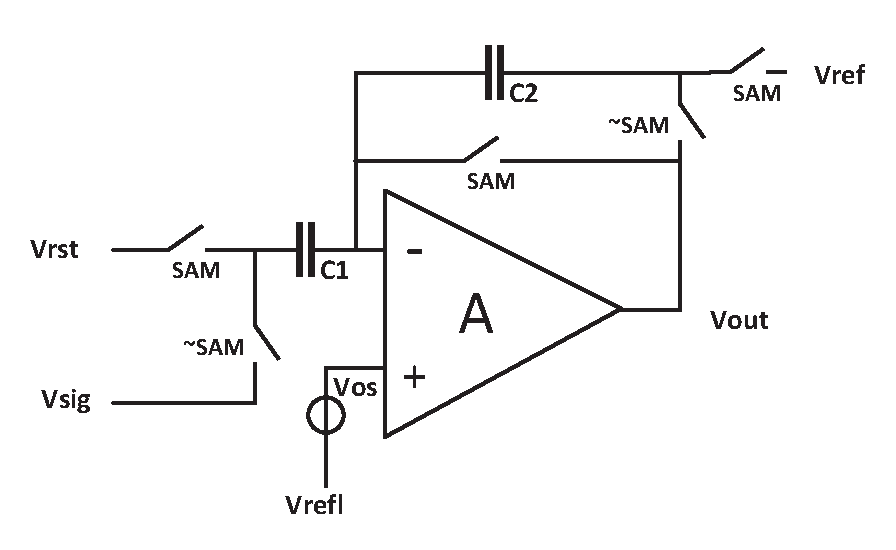
\includegraphics[width=2.5in]{./Figures/CDS.eps}}
	\caption{The structure of the CDS circuits.}
	\label{CDS}
\end{figure} 

\begin{equation}
	\begin{aligned}
		V_{out}&=\left[ V_{ref}+\frac{C_1}{C_2}\ast\left(V_{rst}-V_{sig}\right)\right]\ast\frac{\beta A}{1+\beta A}\\
		&\;{+}\;\left(V\right._{refl}+V_{os})\ast\frac{A}{1+A}\ast\frac{1}{\beta A}\\
		&\;where\ \ \beta=\frac{C_2}{C_1+C_2}
		\label{eq1}
	\end{aligned}
\end{equation}

\subsubsection{Ramp Generator}

As shown in Fig.~\ref{RAMP}, the ramp generator in SS ADC consists of a thermometer-code counter and a capacitor digital-to-analog converter (CDAC). 
While the capacitors in CDAC are being switched one by one from $V_{refl}$ to $V_{vefh}$, the output voltage of the ramp generator is expressed as \eqref{eq2} according to the law of charge conservation. 
In this equation, $N$ represents the number of switched capacitors and $M$ represents the total number of capacitors with the same size (for the 8-bit precision, the total number will be 255). 
Therefore, in PHASE3 (shown in Fig.~\ref{SSWAVE}), the ramp signal changes in stages from $V_{refl}$ to $V_{refh}$, of which the range matches the output of CDS circuits. 
The height of each stage is the least significant Bit (LSB) of the ADC conversion.

The three buffers shown in Fig.~\ref{RAMP} ensure that the reference voltages and ramp signal have sufficient driving capabilities, 
and the output buffer has the largest size in order to drive hundreds of column-parallel comparators.

\begin{figure}[htbp]
	\centerline{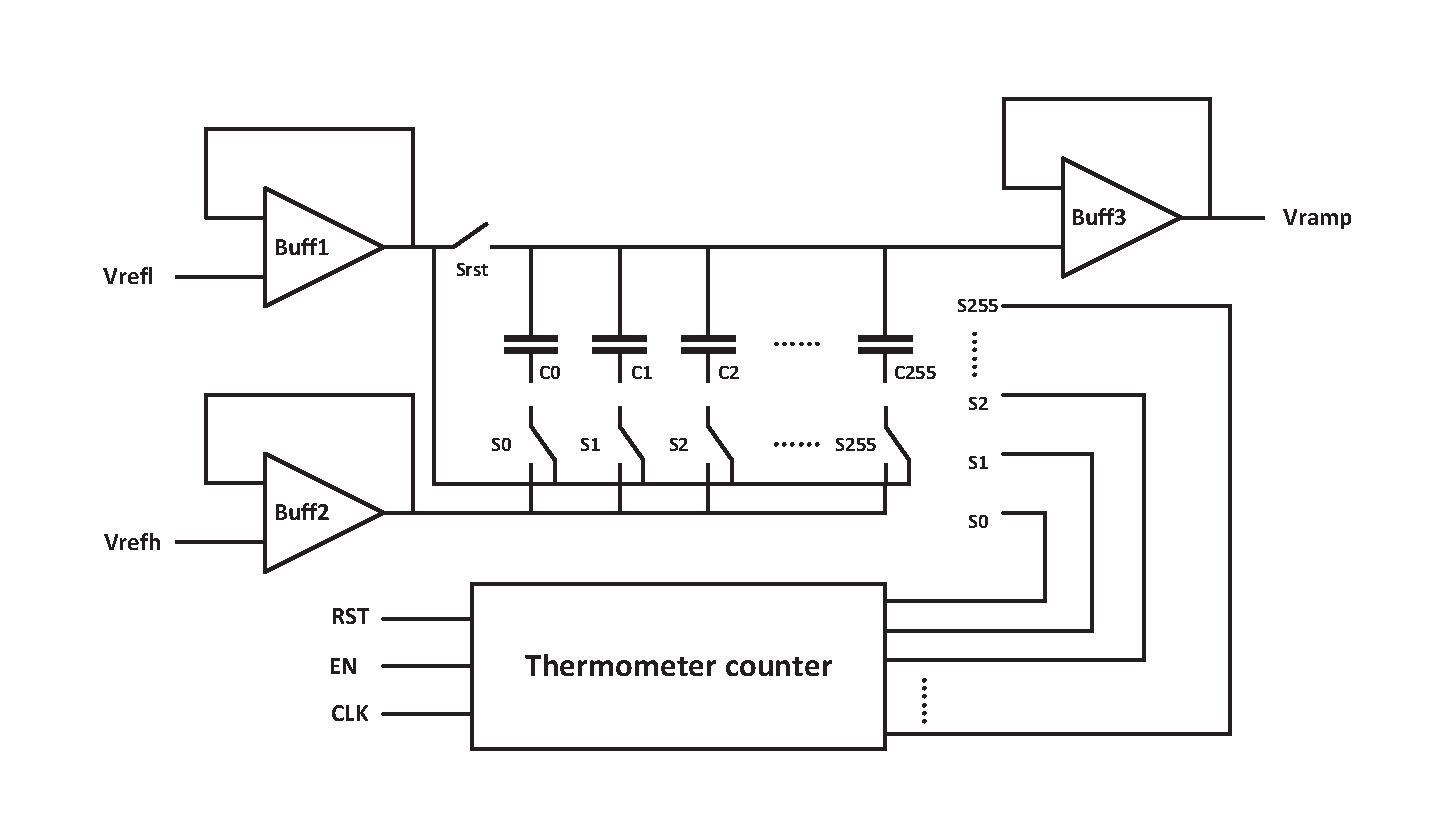
\includegraphics[width=3.5in]{./Figures/RAMP.eps}}
	\caption{The structure of the ramp generator in SS ADC.}
	\label{RAMP}
\end{figure} 

\begin{equation}
	V_{ramp}=V_{refl}+\frac{N}{M}\ast\left(V_{refh}-V_{refl}\right)
	\label{eq2}
\end{equation}

\subsubsection{Comparators}

The comparators are used to compare the CDS circuit output with the ramp signal from the ramp generator. 
In SS ADC, two-stage open-loop comparators can be applied as shown in Fig.~\ref{COM}. According to the law of charge conservation, 
ne
the comparators’ output (PHASE3 shown in Fig.~\ref{SSWAVE}) can be computed as \eqref{eq3}. The comparison is dominated by $V_{ramp}-V_{cds}$ as long as the amplifiers’ open-loop gain 
is large enough while the IOS is also realized.% In addition, the comparators’ speed relies on the bandwidth and slew rate of the amplifiers.

\begin{figure}[htbp]
	\centerline{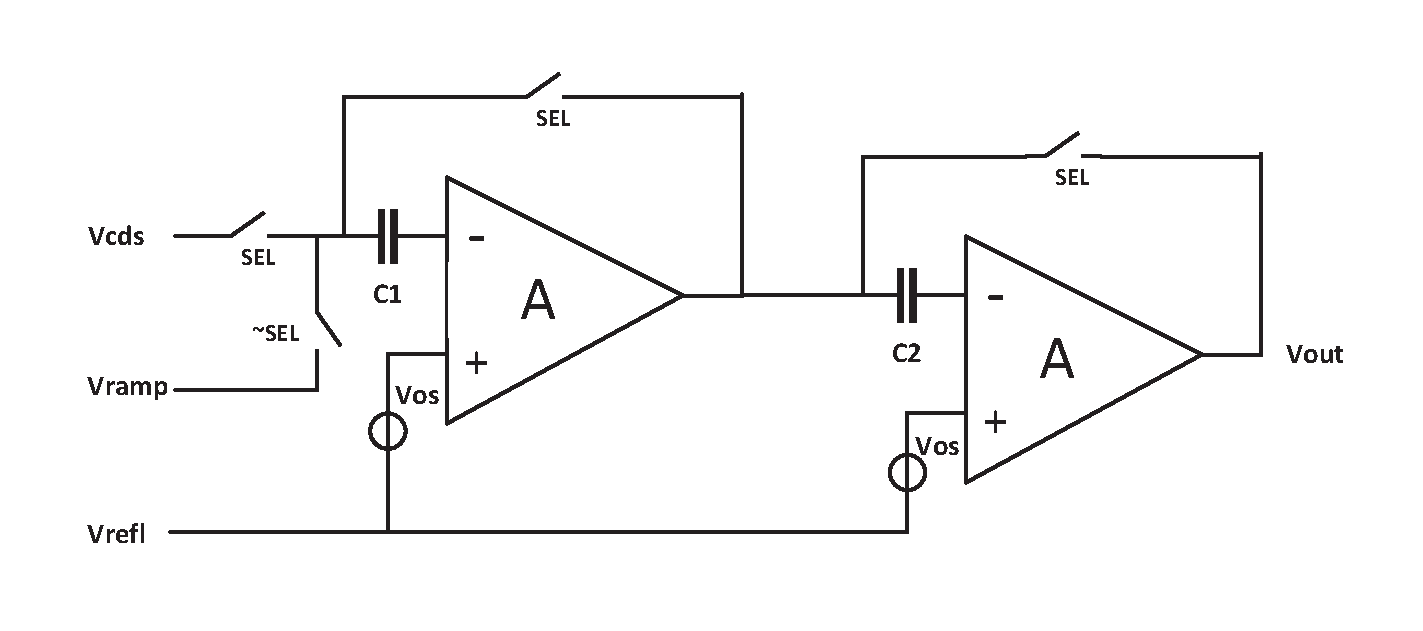
\includegraphics[width=2.5in]{./Figures/COM.eps}}
	\caption{The structure of the comparators in SS ADC.}
	\label{COM}
\end{figure} 

\begin{equation}
	\begin{aligned}
		V_{out}&=A^2(V_{ramp}-V_{cds})\\
		&\;{+}\;\left(V_{refl}+V_{os}\right)\ast\frac{A}{1+A}\\ 		
		\label{eq3}
	\end{aligned}
\end{equation}

\subsection{SAR/SS ADC Architecture Overview}\label{over2}

%Fig.~\ref{SARADC} shows 
The overall architecture of SAR/SS ADC is similar to that of SS ADC shown in Fig.~\ref{SSADC}. The key differences are that the comparators are replaced by low-precision (4bit) SAR sub-ADC, and
the ramp generator is replaced by a resistor digital-to-analog converter (RDAC) with a one-hot code counter.

\iffalse
\begin{figure}[htbp]
  \centerline{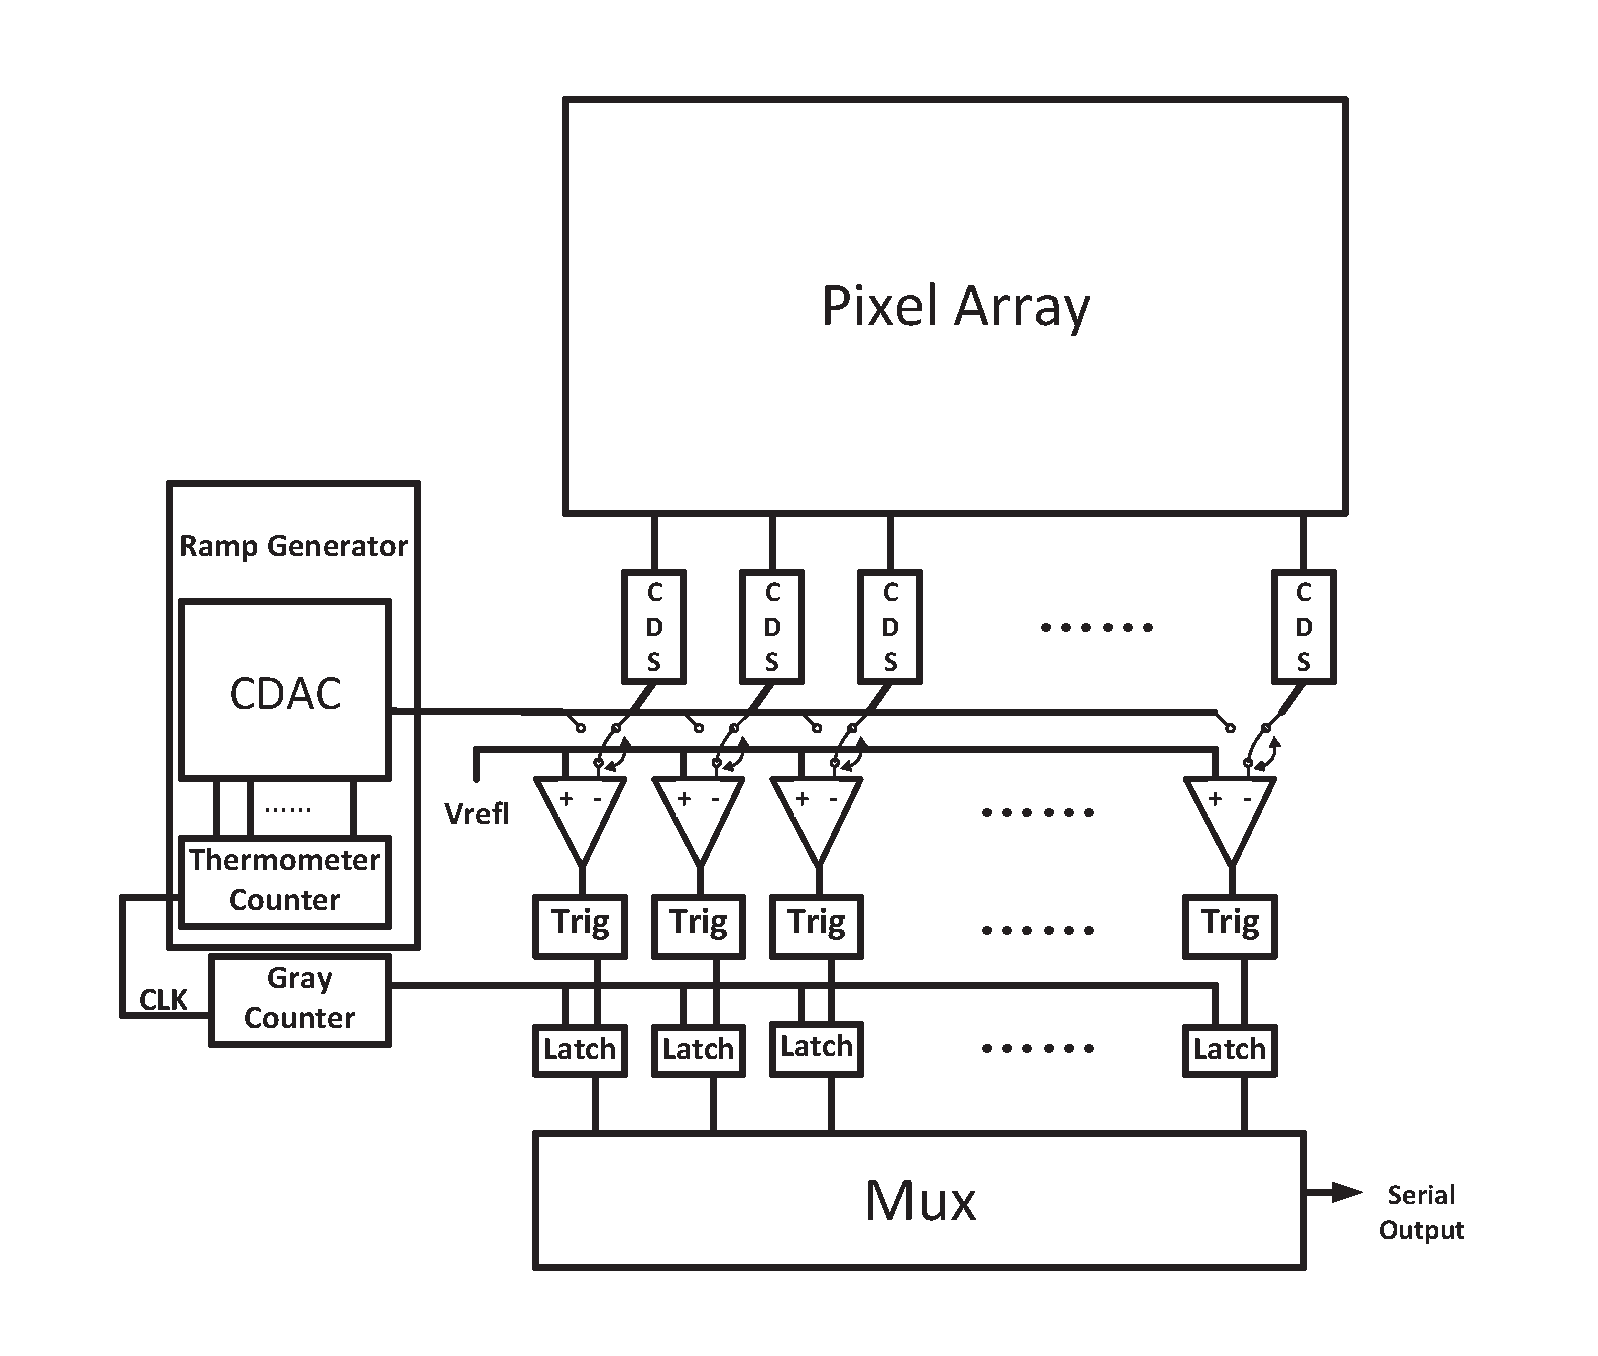
\includegraphics[width=3.5in]{./Figures/SARADC.eps}}
  \caption{Overall architecture of SAR/SS ADC.}
  \label{SARADC}
  \end{figure}
\fi 

As shown in Fig.~\ref{SAR}, a SAR sub-ADC is composed of two input buffers of the reference voltages, an array of digital-to-analog capacitors, a dynamical comparator and a SAR logic block. While generating the upper 4-bit results, $V_{X}$ in SAR sub-ADC is changed according to SAR logic. That means after 4 comparisons 
with the reference voltage, $V_{X}$ is equal to \eqref{eq4}, where $D_{U}\left[\,i\,\right]$ is the $i$ th bit of the upper 4 bits. 
Then the ramp generator starts working, $V_{X}$ then increases gradually as \eqref{eq5}, where $D_{L}\left[\,i\,\right]$ is the $i$ th bit of the lower 6 bits. 
At the time when $V_{X.2}$ exceeds $V_{ref}$, the corresponding $V_{cds}$ is expressed as \eqref{eq6}, which can be represented by the 10-bit conversion results, exactly.

\begin{figure}[htbp]
	\centerline{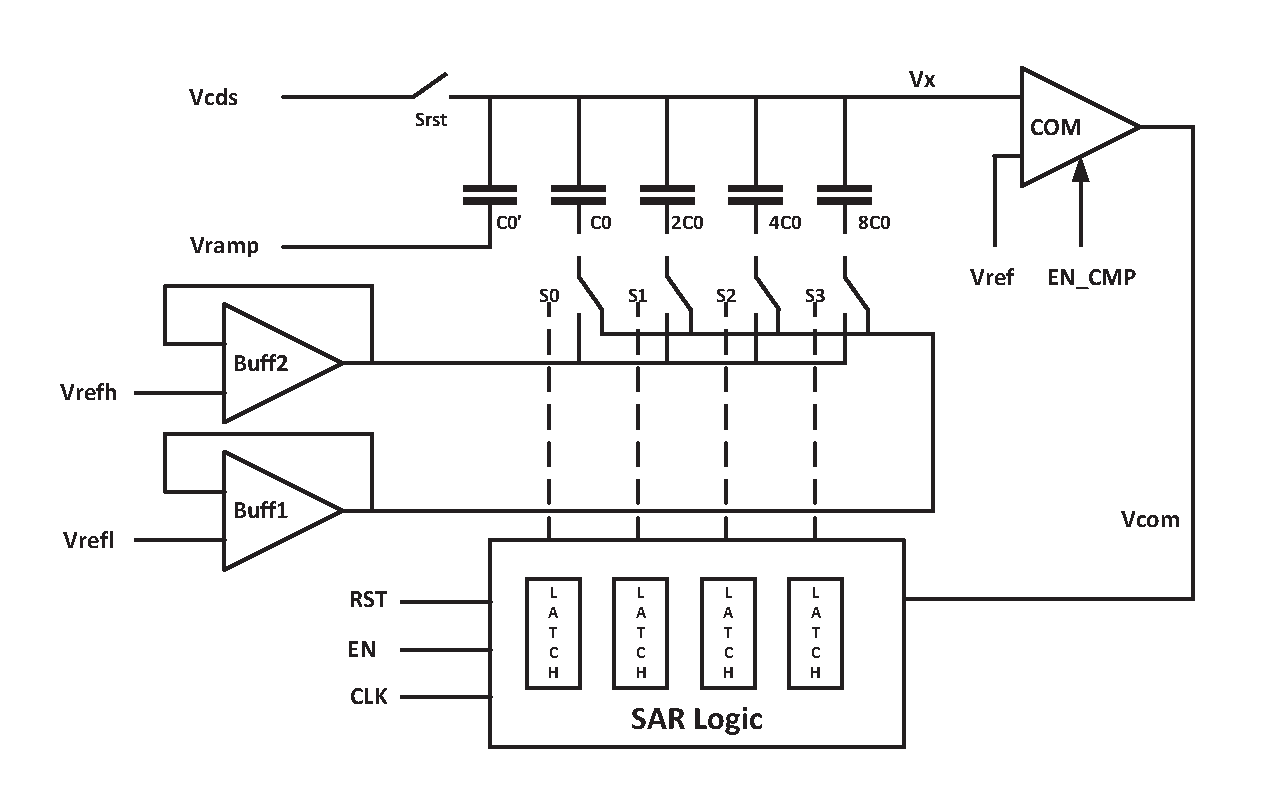
\includegraphics[width=3in]{./Figures/SAR.eps}}
	\caption{The structure of SAR sub-ADCs in SAR/SS ADC.}
	\label{SAR}
\end{figure}

\begin{equation}
	V_{X.1}=V_{cds}+\sum_{i=1}^{4} {\frac{V_{ref}}{2^{i}}\ast{D_{U}\left[\,i\,\right]}}
	\label{eq4}
\end{equation}

\begin{equation}
	\begin{aligned}
		&V_{X.2}=V_{X.1}+\frac{V_{ramp}}{2^4}\\ &where\  V_{ramp}=\frac{V_{ref}}{2^6-1}\ast\sum_{i=1}^{6}2^{6-i}\ast{D_{L}\left[\,i\,\right]}
		\label{eq5}
	\end{aligned}	
\end{equation}

\begin{equation}
	\begin{aligned}
		&V_{cds}=k\ast(V_{rst}-V_{sig})\\
		&\;{\approx}\;{V_{ref}-\sum_{i=1}^{4} \frac{V_{ref}}{2^{i}}\ast{D_{U}\left[\,i\,\right]}-\sum_{i=1}^{6} \frac{V_{ref}}{2^{4+i}}\ast{D_{L}\left[\,i\,\right]}}
		\label{eq6}
	\end{aligned}
\end{equation}

It is worth noting that we assign 14 steps for the 4 comparisons with SAR logic (in SAR/SS ADC, we define 1 clock step as 2 clock periods, which is 100ns). Both the first and second comparison takes 4 steps and the following two comparison takes 3 steps. It is because that the more rapidly $V_{X}$ can be changed, the more time it may be required for comparison. As for the last comparison with SS logic, 1 step is sufficient because $V_{X}$ will not exceed $V_{ref}$ rapidly, allowing the comparators to response in-time.

Fig.~\ref{RRAMP} shows the structure of the ramp generator in SAR/SS ADC, which consists of an R-string made up of 68 unit resistors. $V_{ramp}$ has a total number of 68 steps,
of which 64 steps with a step size of $(V_{refh}-V_{refl})/64$ are used to generate the lower 6-bit results and 4 redundant steps are used to ensure that the comparators 
will always be flipped to latch the results. During operation, $V_{0}$ to $V_{67}$ in the ramp generator is sequentially selected as the output and thereby 
$V_{ramp}$ is changed from $V_{vefl}$ to $V_{vefl}+17/16(V_{refh}-V_{refl})$.

\begin{figure}[htbp] 
	\centerline{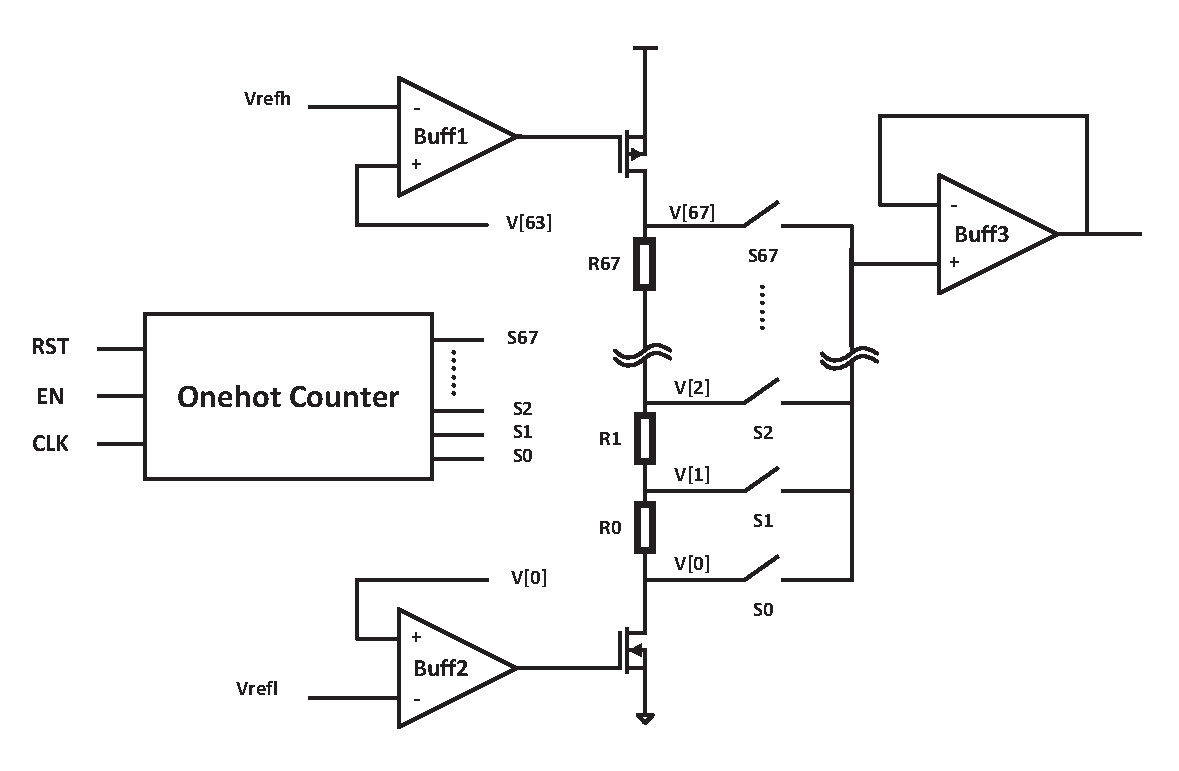
\includegraphics[width=2.5in]{./Figures/RRAMP.eps}}
	\caption{The structure of the ramp generator in SAR/SS ADC.}
	\label{RRAMP}
\end{figure}

Compared to CDAC, RDAC is able to generate the ramp signal without the gain error caused by the input capacitors of the output buffer, 
which is necessary to achieve 10-bit precision in SAR/SS hybrid architecture.
Besides, the two buffers of the reference voltages in the RDAC require less energy than those in the CDAC due to less load capacitance.  

The related operational waveform of SAR/SS ADC is shown in Fig.~\ref{SARWAVE}. The upper 4-bit results (as the second last item of \eqref{eq6}) are generated 
with SAR logic and the lower 6-bit results (as the last item of \eqref{eq6}) are counted according to the time between the ramp signal’s start and the comparators’ last flip. 

\begin{figure}[htbp]
	\centerline{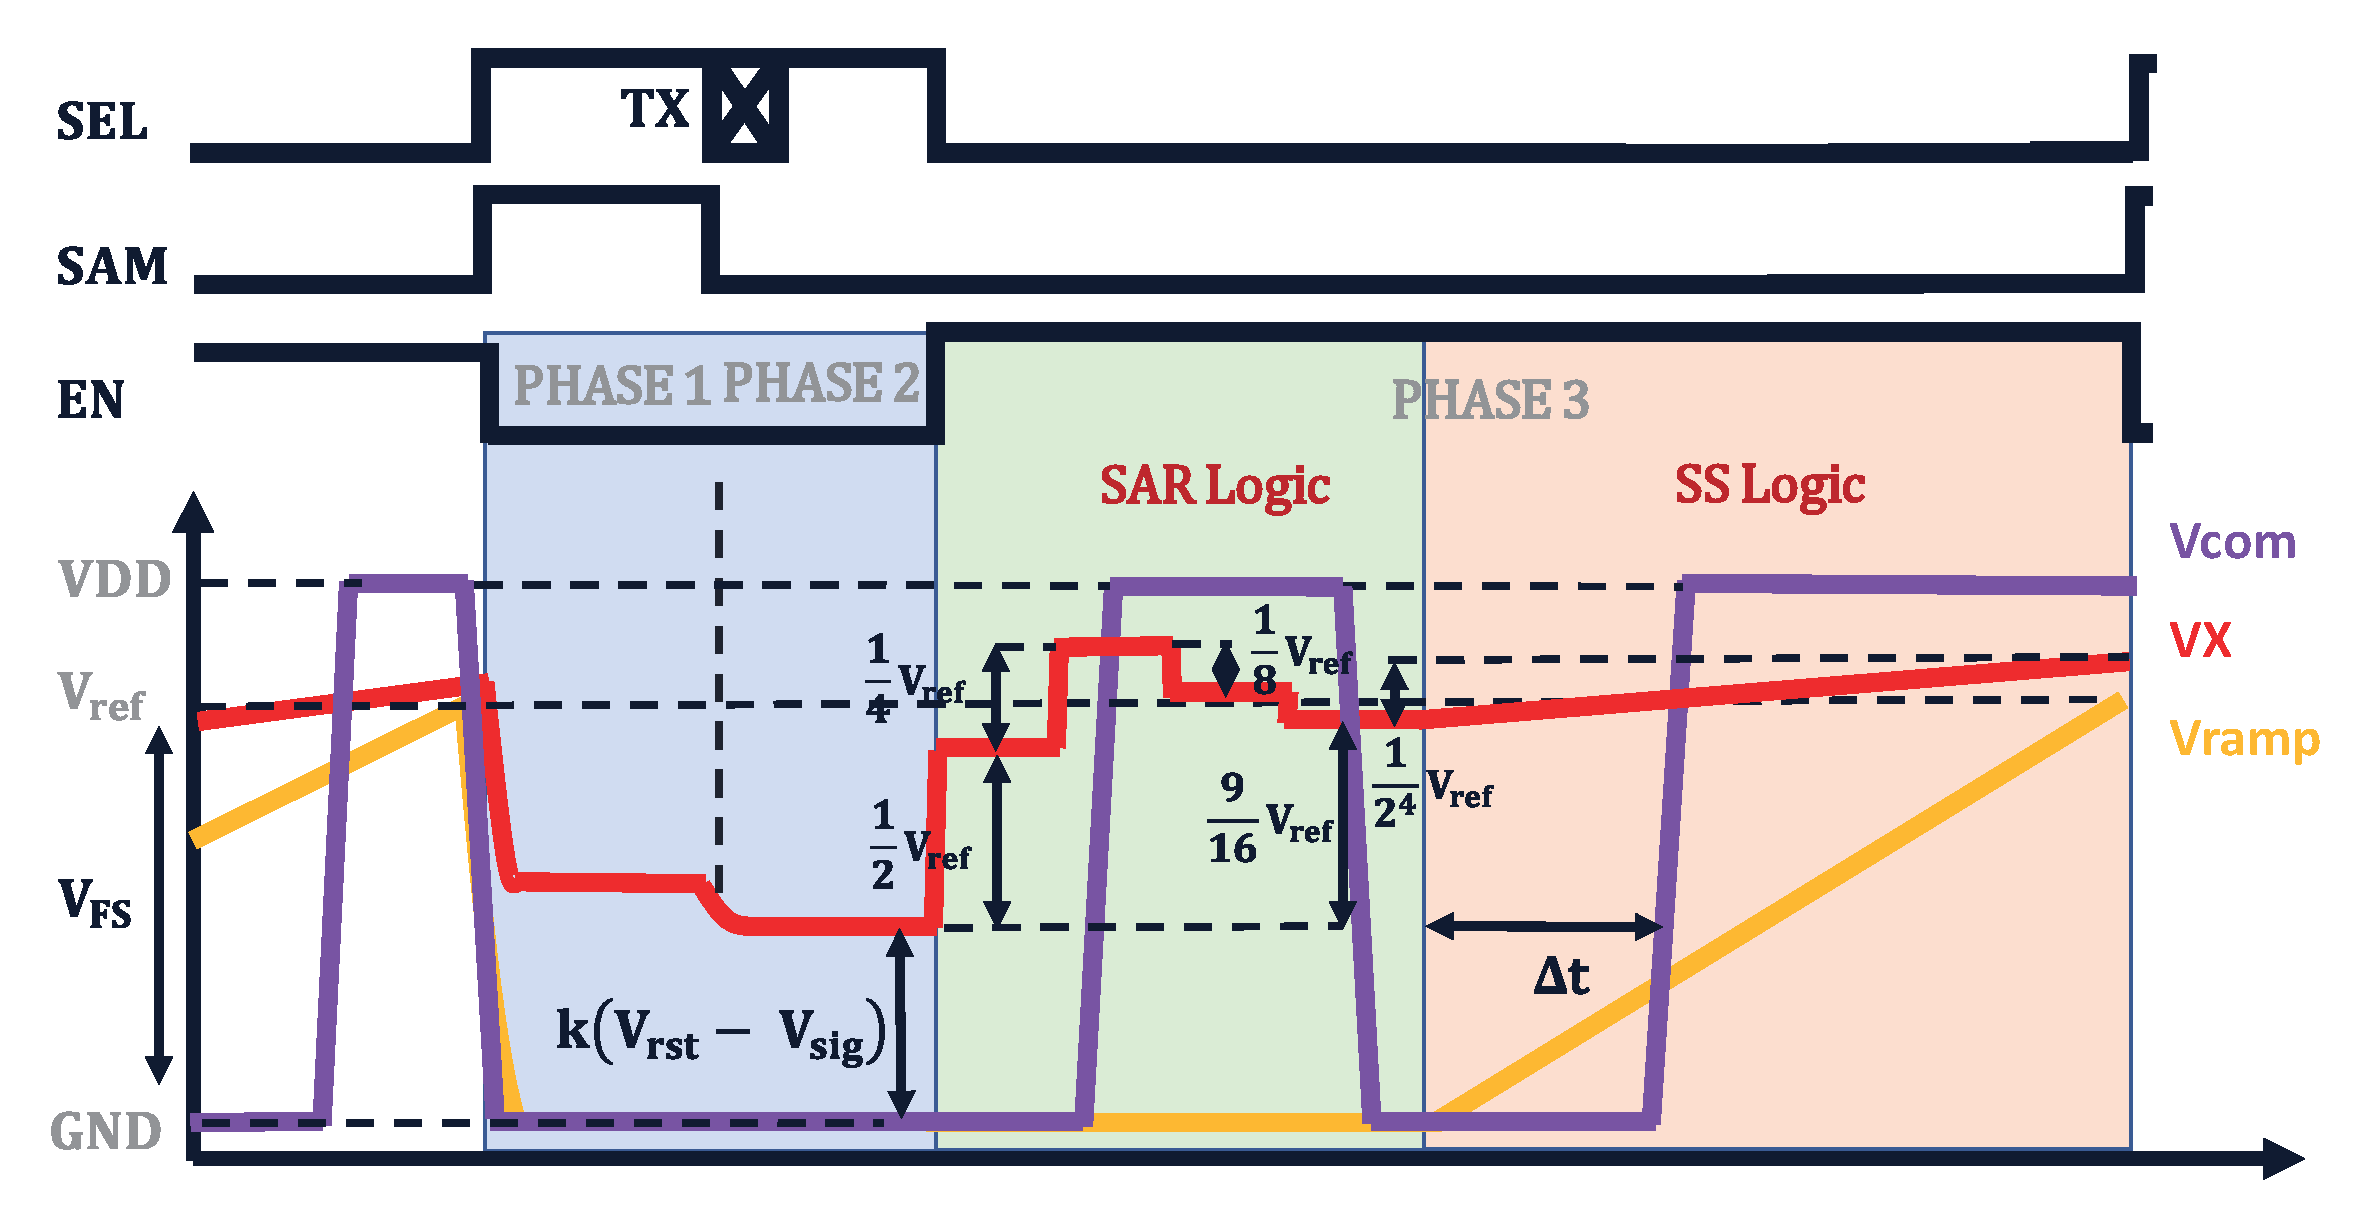
\includegraphics[width=3.5in]{./Figures/SARWAVE.eps}}
	\caption{The operational waveform of SAR/SS ADC.}
	\label{SARWAVE}
\end{figure} 

As for the dynamical comparators inside SAR sub-ADC, a strong-arm comparator with pre-amplifiers can be used as shown in Fig.~\ref{LATCH}. Such comparators 
are suitable for multiple comparisons because high speed is easily achieved and every comparison is under the control of the clock. Besides, the offset voltages of the pre-amps can be effectively eliminated by output offset cancellation (OOS) \cite{razavi_design_1992}.

\begin{figure}[htbp]
	\centerline{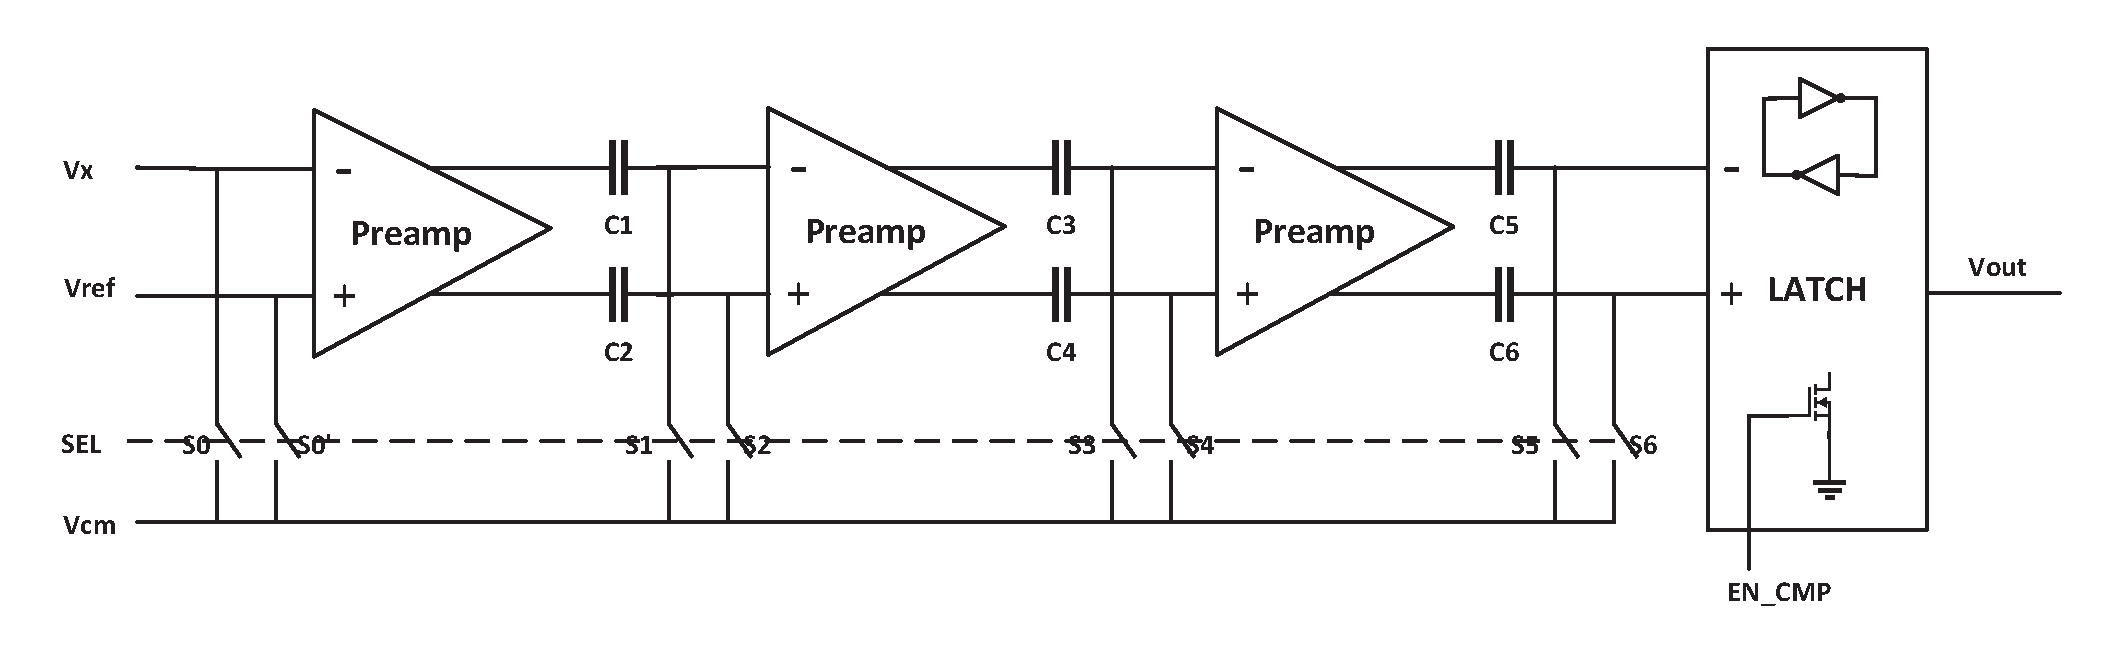
\includegraphics[width=3.5in]{./Figures/LATCH.eps}}
	\caption{The structure of the comparators in SAR sub-ADCs.}
	\label{LATCH}
\end{figure} 

The design decision regarding 4/8-bit adaptive-precision for SS ADC and 4/10-bit adaptive-precision for SAR/SS ADC is discussed in Sect.~\ref{discussion}.

%\subsection{Power Gating and Adaptive-Precision Implementation}\label{strategy}

\subsection{Implementation of Power Gating}\label{gating1}

As shown in  Fig.~\ref{GATING}, the proposed power gating method is implemented by adding PMOS-transistor switches between the functional blocks and the supply voltage \cite{keating_low_2007}. 
When the switches are turned off, the corresponding blocks’ current paths are cut off and the energy is saved. 

Fine-grain power gating is beneficiary to power and energy savings. On the other hand, 
to avoid unacceptable IR drop, the area overhead of the switch circuit may be significant, 
and inverters need to be inserted between the control signal and the switching gates for 
sufficient driving capabilities. 

In addition, the longer the functional blocks is powered off, the better power scaling benefit can be obtained. Therefore, for power gating, continuous long periods of time are preferred than individual short periods of time, since block shutdown and recovery times should also be considered.
As shown in Fig.~\ref{TIME}, due to the shutdown and recovery time of the function block, frequent 
power gating over short time intervals may introduce extra overhead. 

Since column-parallel ADC not only has high column-parallel current that can be controlled, but also offers continuously and exponentially long power-off time intervals thanks to the widely adopted SS conversion logic, applying power gating to this architecture is highly efficient.

\begin{figure}[htbp]
	\centerline{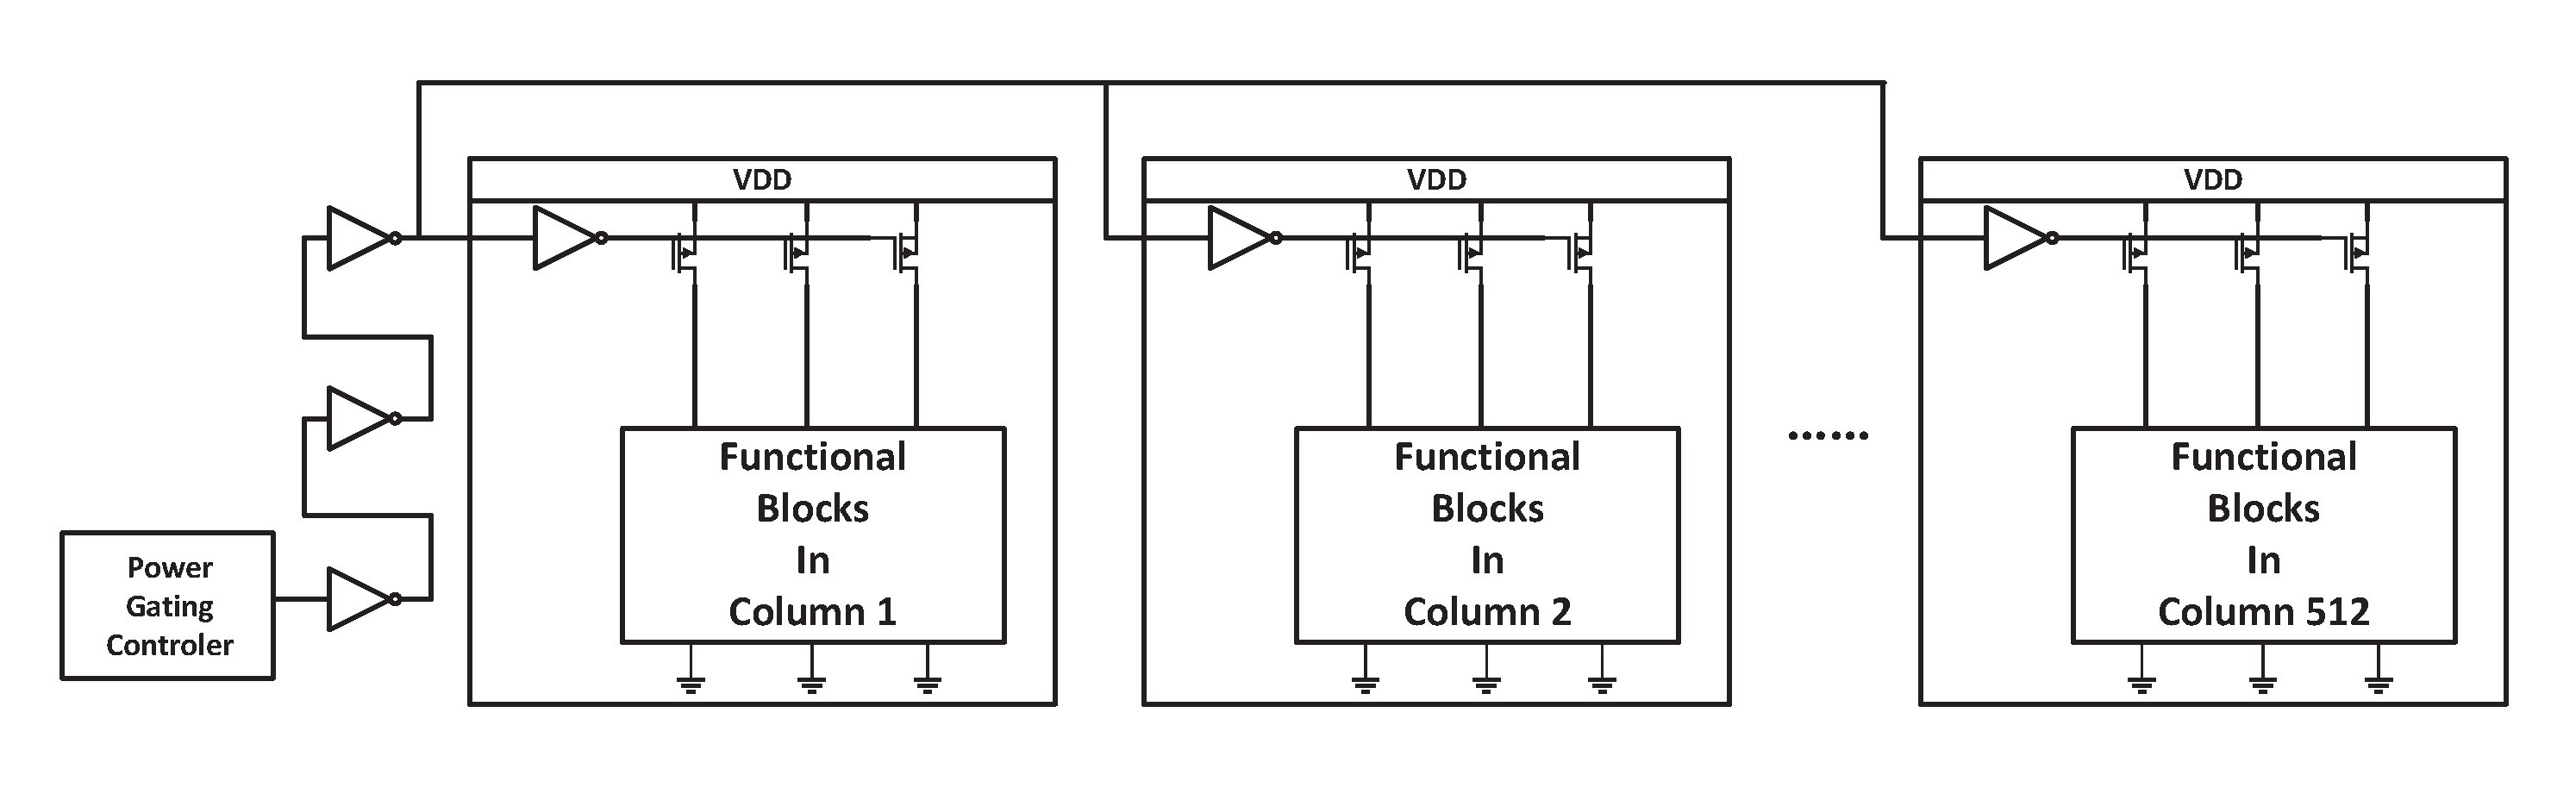
\includegraphics[width=3.5in]{./Figures/GATING.eps}}
	\caption{Implementation of power gating.}
	\label{GATING}
\end{figure} 

\begin{figure}[htbp]
	\centerline{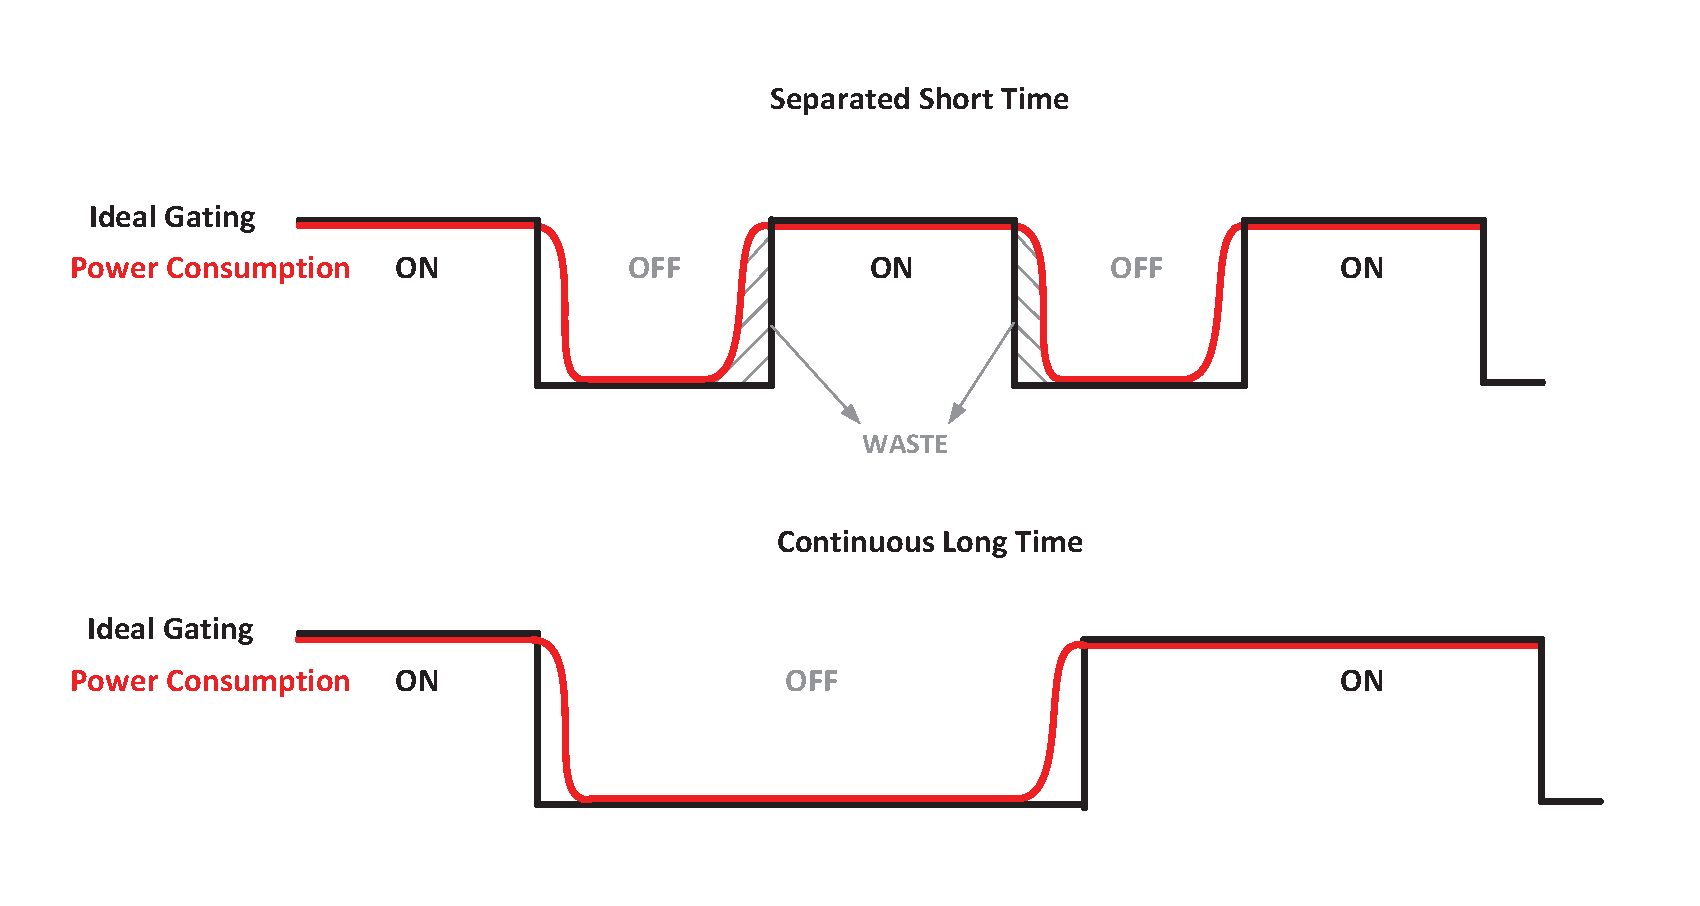
\includegraphics[width=3.5in]{./Figures/TIME.eps}}
	\caption{Continuous long time versus separated short time for power gating.}
	\label{TIME}
\end{figure}  

\subsection{Adaptive-Precision Implementation for SS ADC}\label{gating2}

As evaluated in Sect.~\ref{result}, SS ADC power consumption is mainly taken up by the column-parallel comparators, bias circuits, and the output buffer of the ramp generator. 
Considering that all bias circuits are settled down only once (tens of microseconds after the whole system is powered up) and then other circuits can be settled down quickly by the distributed 
bias circuits, we only apply power gating to the amplifiers in the comparators and the output buffer in the ramp generator.

For low-precision conversion, the thermometer-code counter should be extended to support switching the capacitors in CDAC 16 by 16 instead of one by one and thereby the ramp signal can reach $V_{refh}$ in 16 steps (for 4 bits) instead of in 256 steps (for 8 bits). 
After the 16 steps, the comparators and the output buffer can be powered off for an extended period of time, leaving the related signals decrease gradually.
The related waveform are shown in Fig.~\ref{SS_pg}. 

\begin{figure}[htbp]
	\centerline{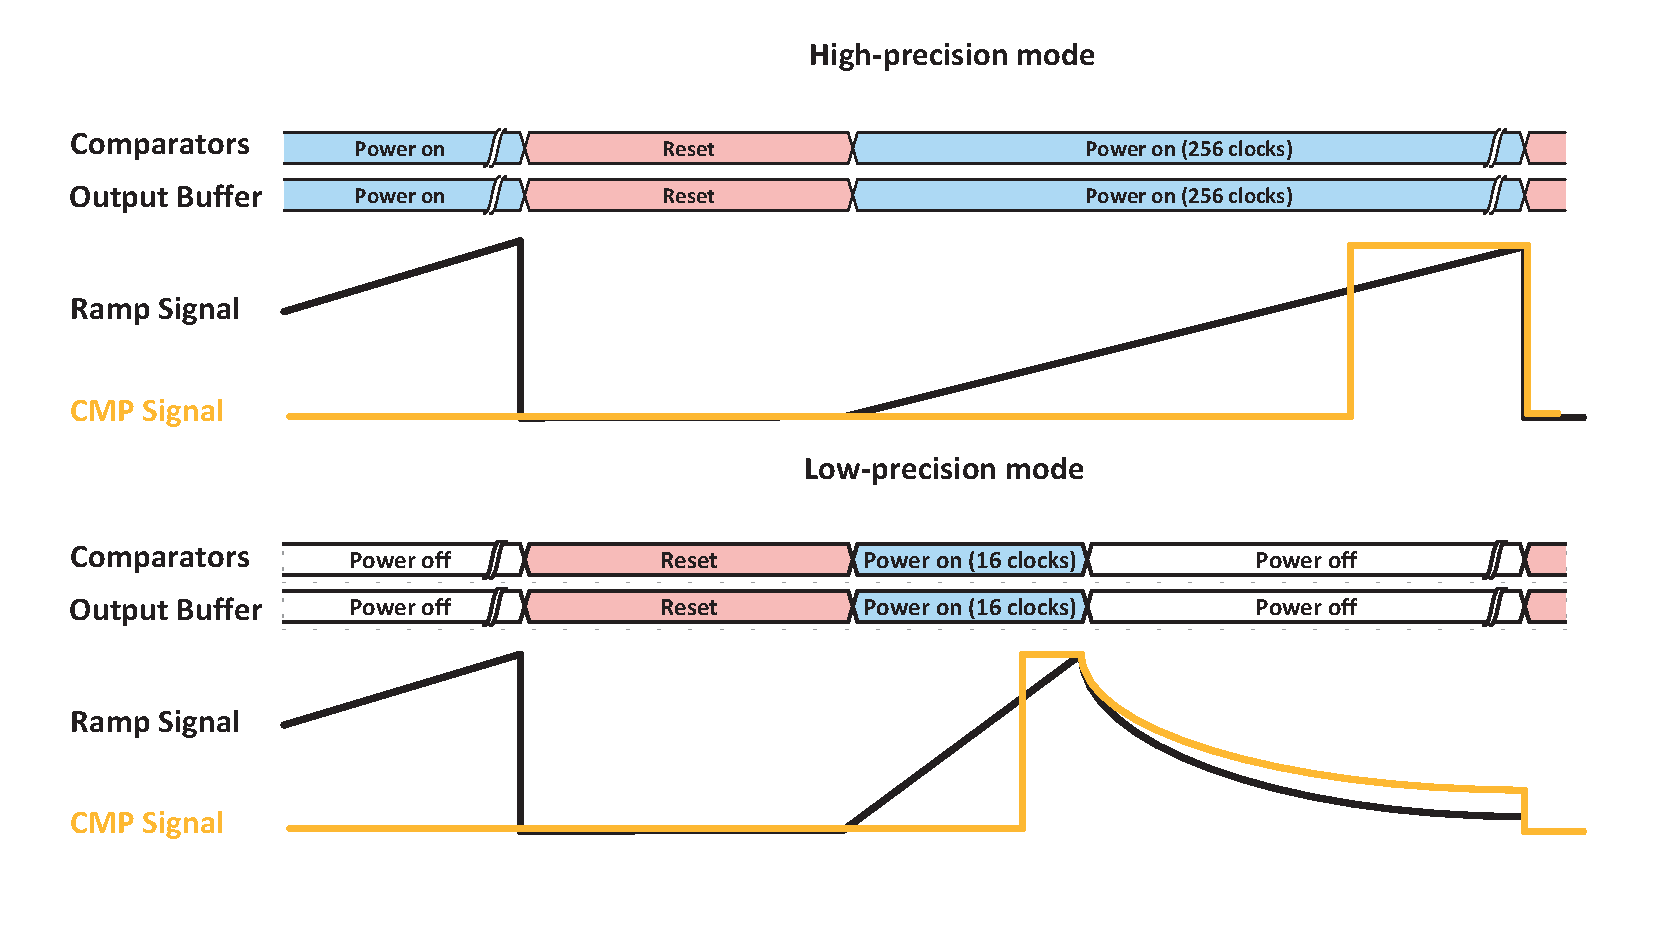
\includegraphics[width=3.2in]{./Figures/SS_pg.eps}}
	\caption{Adaptive-precision and power gating implementation for SS ADC.}
	\label{SS_pg}
\end{figure} 

To avoid the decreasing output of comparators causing extra unwanted latch for the low-precision conversion results, an NMOS switch and a PMOS switch are inserted into the two inverters following the comparator as shown in Fig.~\ref{MATE}. 
For high-precision conversion, the gating signal will be low-level and turn on the PMOS switch, thus the second inverter output will be the same as the comparator output, which is either low-level or high-level. 
For low-precision conversion, the NMOS switch is turned on by the high-level gating signal and the second inverter input is connected to the ground. Therefore, the output signal of the two inverters will remain high-level, preventing unpredictable latch caused by the comparator metastable output.

\begin{figure}[htbp]
	\centerline{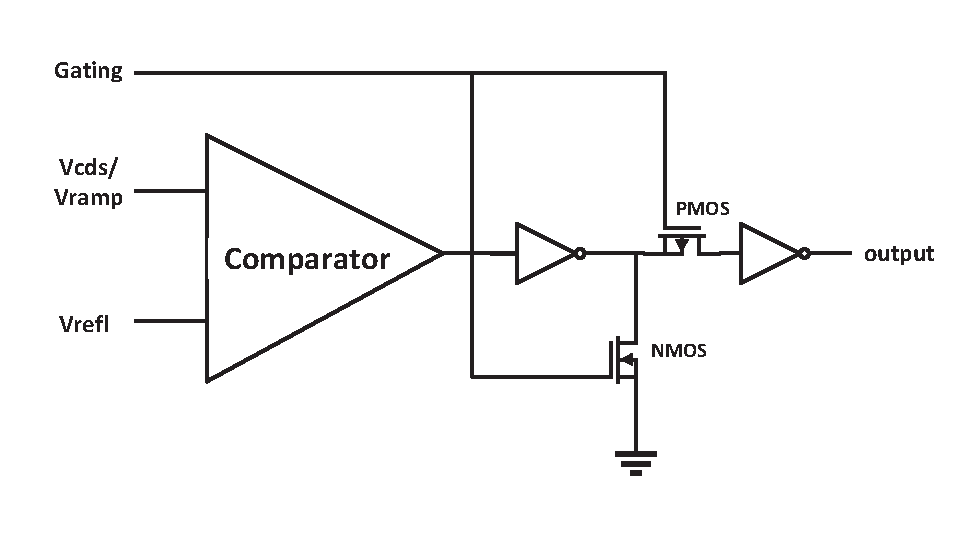
\includegraphics[width=2.5in]{./Figures/MATE.eps}}
	\caption{Two switches added to the inverters following the comparator in SS ADC.}
	\label{MATE}
\end{figure} 

\subsection{Adaptive-Precision Implementation for SAR/SS ADC}\label{gating3}

As evaluated in Sect.~\ref{result}, SAR/SS ADC power consumption is mainly contributed by the column-parallel buffers of reference voltages in SAR sub-ADC.
It is because that these buffers need to drive relatively large and changing load capacitance, with relatively large static and dynamical current.
Therefore, gating these buffers will significantly reduce both static power consumption and dynamical power consumption for the ADC.

In addition, the CDS circuits and comparators in SAR/SS ADC also consume a significant amount of energy. However, we only choose to take the comparators under control because they can conveniently share the same gating signal with the buffers. And the gating signal of the buffers can also be the same as the start signal of the ramp generator. Therefore, gating the buffers and comparators in SAR/SS ADC introduces limited extra control logic with a few shared level-shifters and inverters.

Furthermore, the power distribution results shown in Sect.~\ref{result} demonstrate that adaptive-precision tuning is unnecessary within the ramp generator of SAR/SS ADC, which means the counter in SAR/SS ADC do not need to support two modes for adaptive-precision as in SS ADC.

The signal waveform is shown in Fig.~\ref{SAR_pg}. As we can see, for low-precision conversion, the SAR buffers and comparators are power gated. Therefore, although the ramp signal is generated as usual, the 4-bit results will be completely generated by the SAR logic. 

\begin{figure}[htbp]
	\centerline{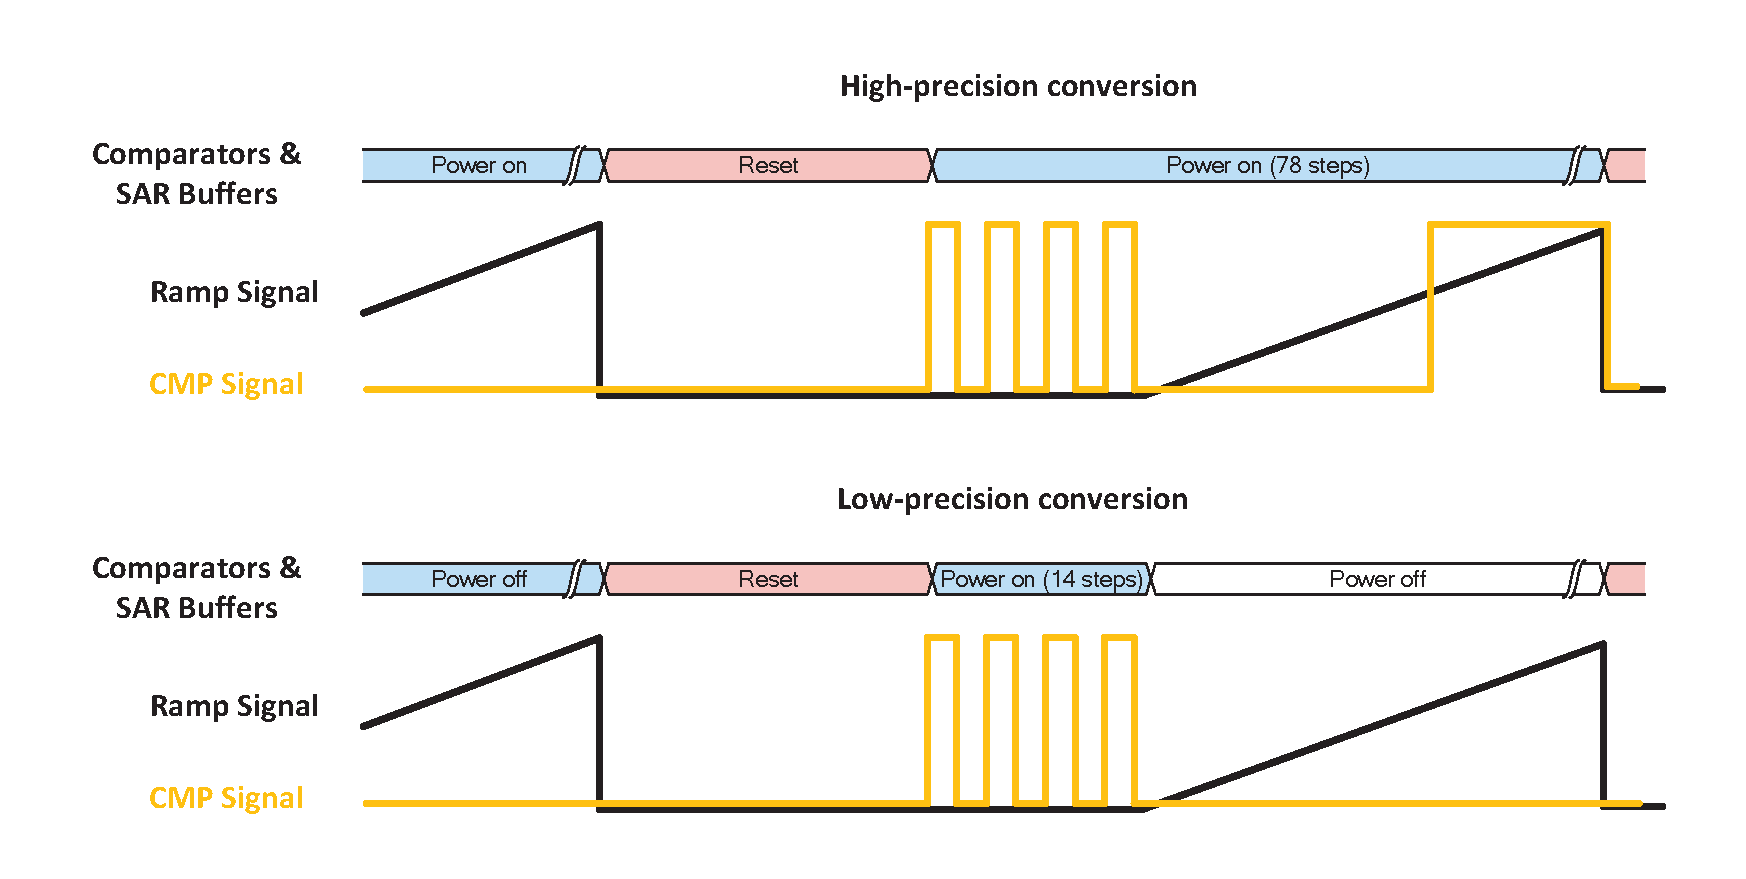
\includegraphics[width=3.5in]{./Figures/SAR_pg.eps}}
	\caption{Adaptive-precision and power gating implementation for SAR/SS ADC.}
	\label{SAR_pg}
\end{figure} 

	%\section{Implementation of Adaptive Precision and Power Gating}\label{strategy}

\subsection{Implementation of Power Gating}

The power gating can be implemented simply by adding PMOS-transistor switches between the functional blocks and the supply voltage \cite{keating_low_2007} as presented in Fig.~\ref{GATING}. 
When the switches are turned off, the corresponding blocks’ current paths will be cut off and thereby the energy is saved. 

It is obvious that for analog circuits, the more current is under control, the more effective the power gating can be. However, to avoid unacceptable IR drop, the total size of the switches may be large, 
and inverters should be inserted between the control signal and the switches’ gates for sufficient driving capability. 

Besides, the longer time the functional blocks can be power off, the better power scaling capacity can be obtained. And a continuous long time is preferred than separated short time for power gating because the blocks' metastability should also be taken into consideration.
As presented in Fig.~\ref{TIME}, separated short time for power gating will inevitably waste more
time for the blocks' shut down or recovery. 

As the collumn-parallel ADCs not only have large amounts of column-parallel currents that can be controlled, but also offer continuously and exponentially scalable power-off time thanks to the widely adopted SS conversion logic, applying power gating to this architecture will be highly promising.

\begin{figure}[htbp]
	\centerline{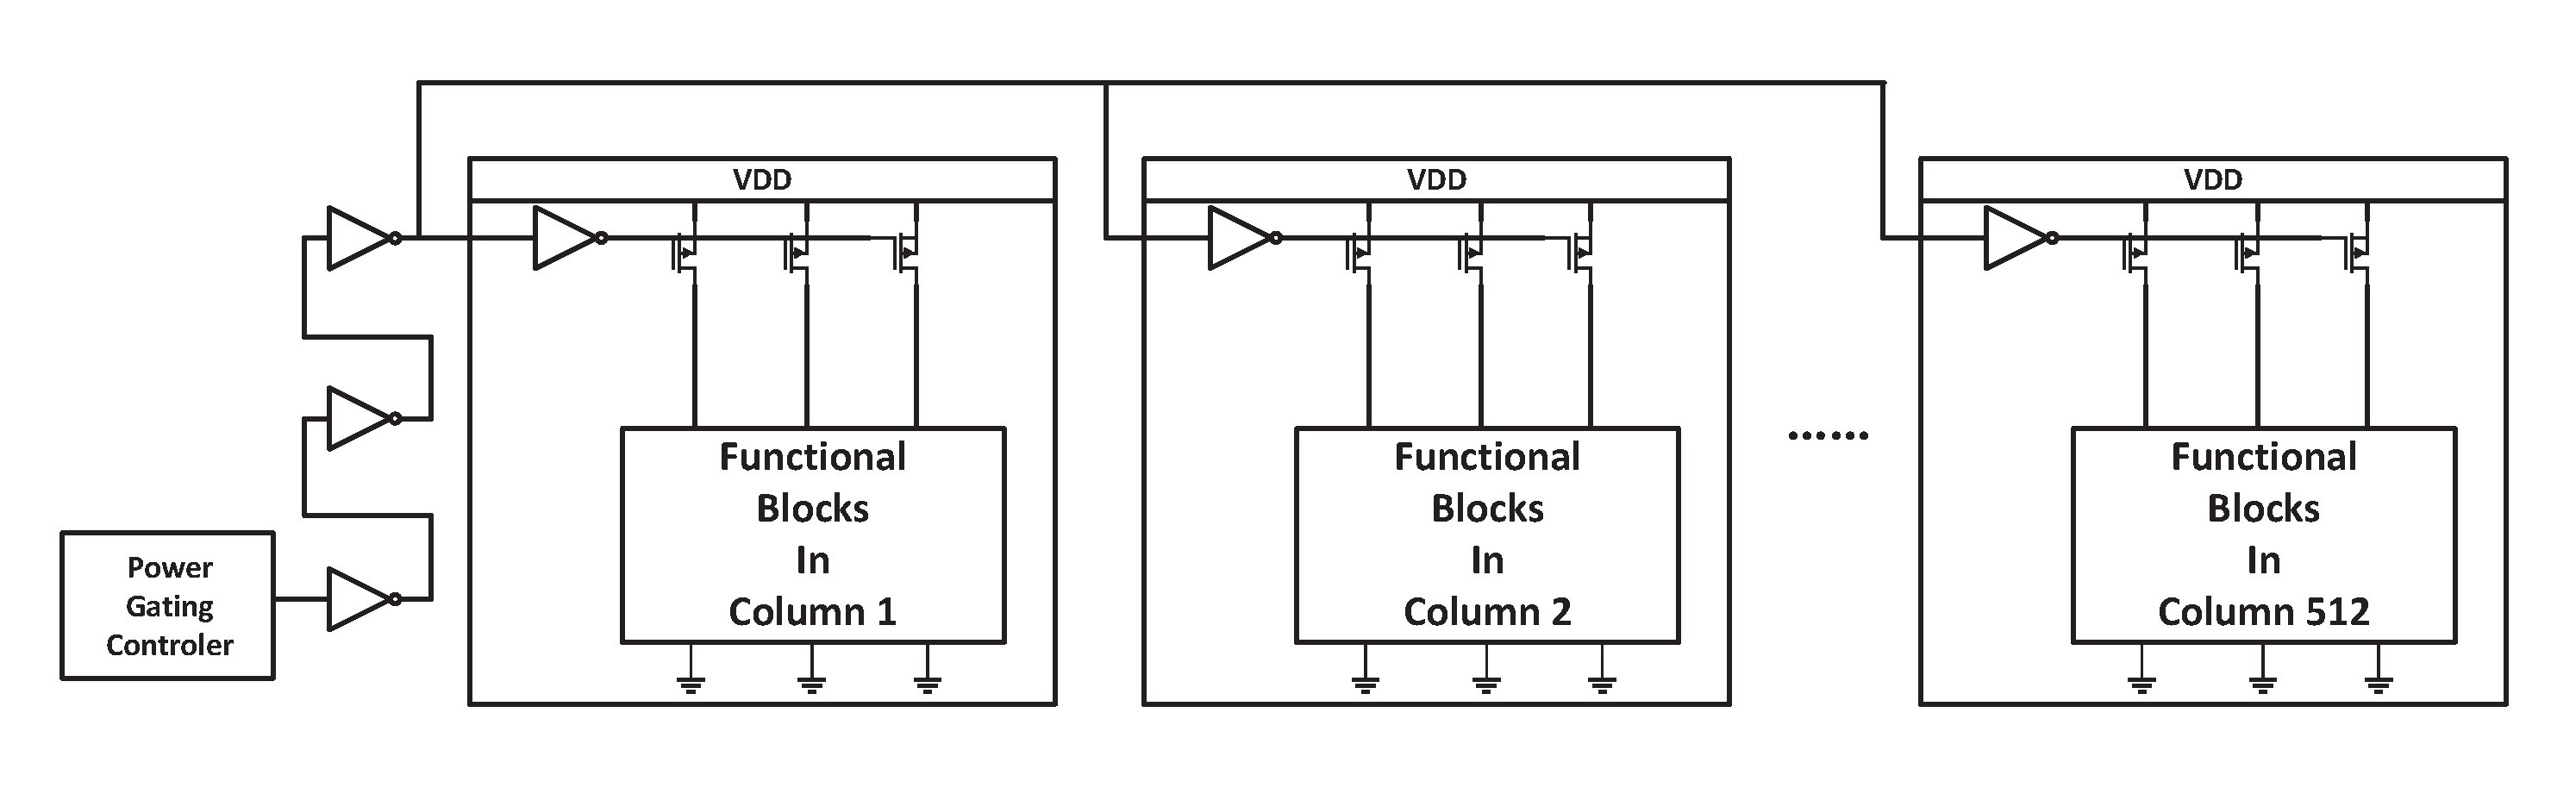
\includegraphics[width=3.5in]{./Figures/GATING.eps}}
	\caption{Implementation of Power Gating}
	\label{GATING}
\end{figure} 

\begin{figure}[htbp]
	\centerline{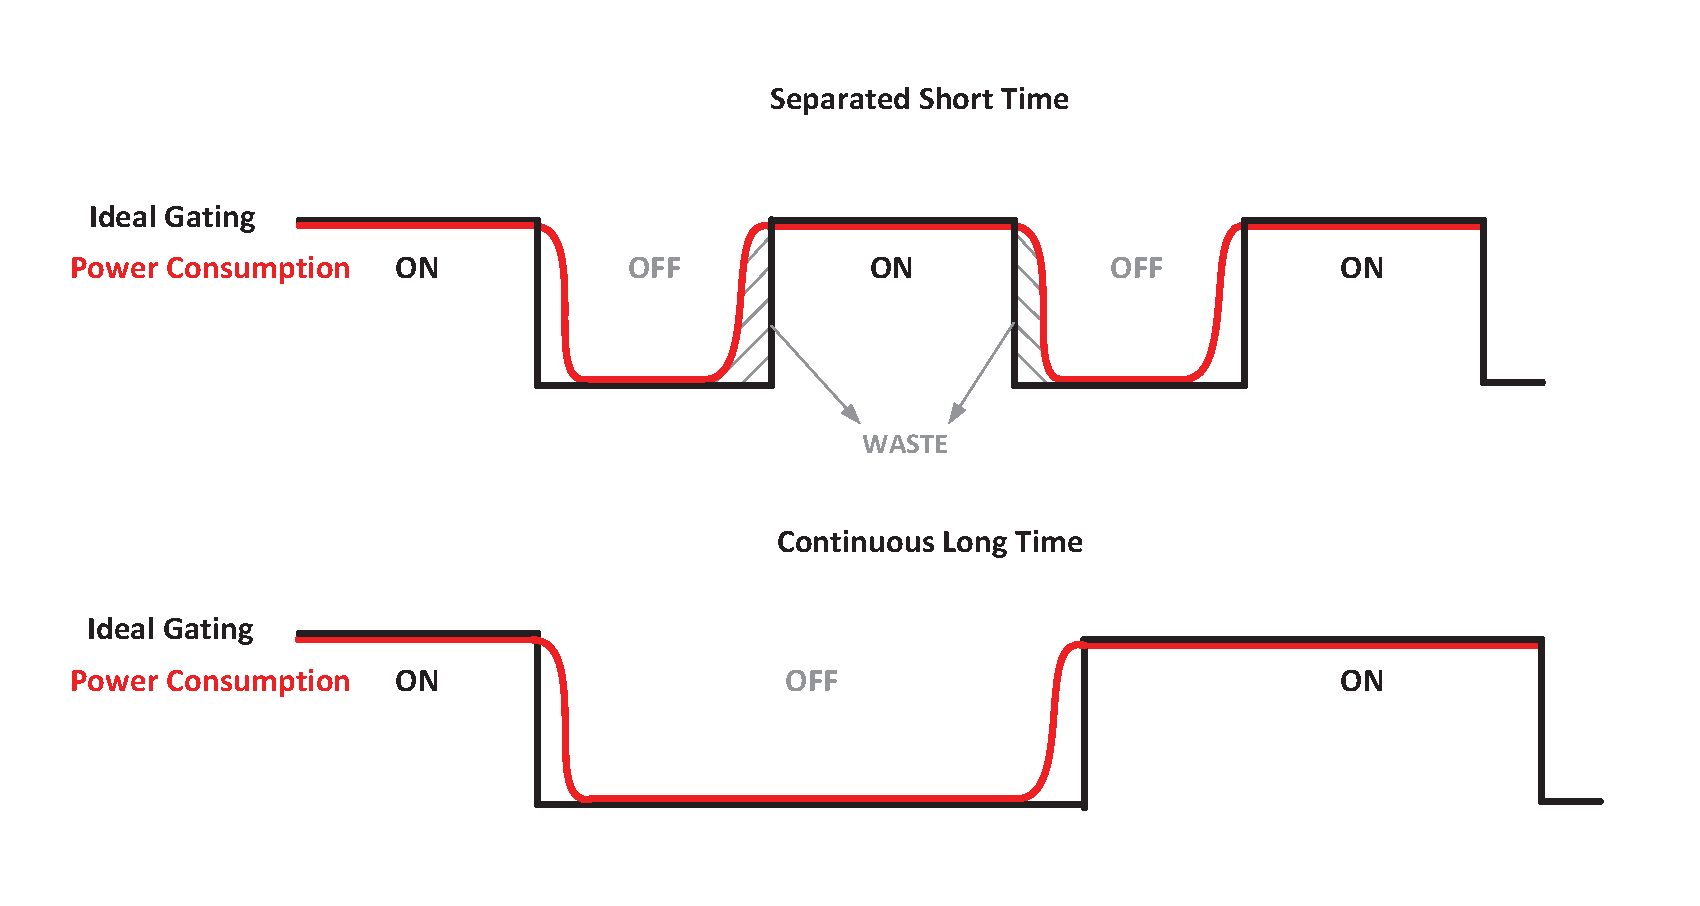
\includegraphics[width=3.5in]{./Figures/TIME.eps}}
	\caption{Continuous Long Time versus Separated Short Time for Power Gating.}
	\label{TIME}
\end{figure}  

\subsection{Implementation for the SS ADCs}

As evaluated in Sect.~\ref{result}, the SS ADCs’ power consumption is mainly taken up by the column-parallel comparators, bias circuits, and the output buffer of the ramp generator. 
Considering that all bias circuits are settled down only once (tens of microseconds after the whole system's power up) and then other circuits can be settled down quickly by the distributed 
bias circuits, we just apply power gating to the amplifiers in the comparators and the output buffer in the ramp generator.

For low-precision conversion, the thermometer counter should have been extended to support switching the capacitors in CDAC 16 by 16 instead of one by one and thereby the ramp signal can reach $V_{refh}$ in 16 steps (for 4 bits) instead of in 256 steps (for 8 bits). 
After the 16 steps, the comparators and the output buffer can be power off for an extented period of time, leaving the related signals decrease gradually.
The related waveform are presented in Fig.~\ref{SS_pg}. 

To avoid the decreasing output of comparators causing extra unwanted latch for the low-precision conversion results, an NMOS switch and a PMOS switch are added to the two inverters fowllowing the comparator as presented in Fig.~\ref{MATE}. 
For high-precision conversion, the gating signal will be low-level and turn on the PMOS switch, thus the second inverter's output will be the same as the comparator's output, which is either low-level or high-level. 
For low-precision conversion, the NMOS switch is turned on by the high-level gating signal and the second inverter's input is connected to the ground. Therefore, the output signal of the two inverters will remain high-level, preventing unpredictable latch caused by the comparator's metastable output.

\begin{figure}[htbp]
	\centerline{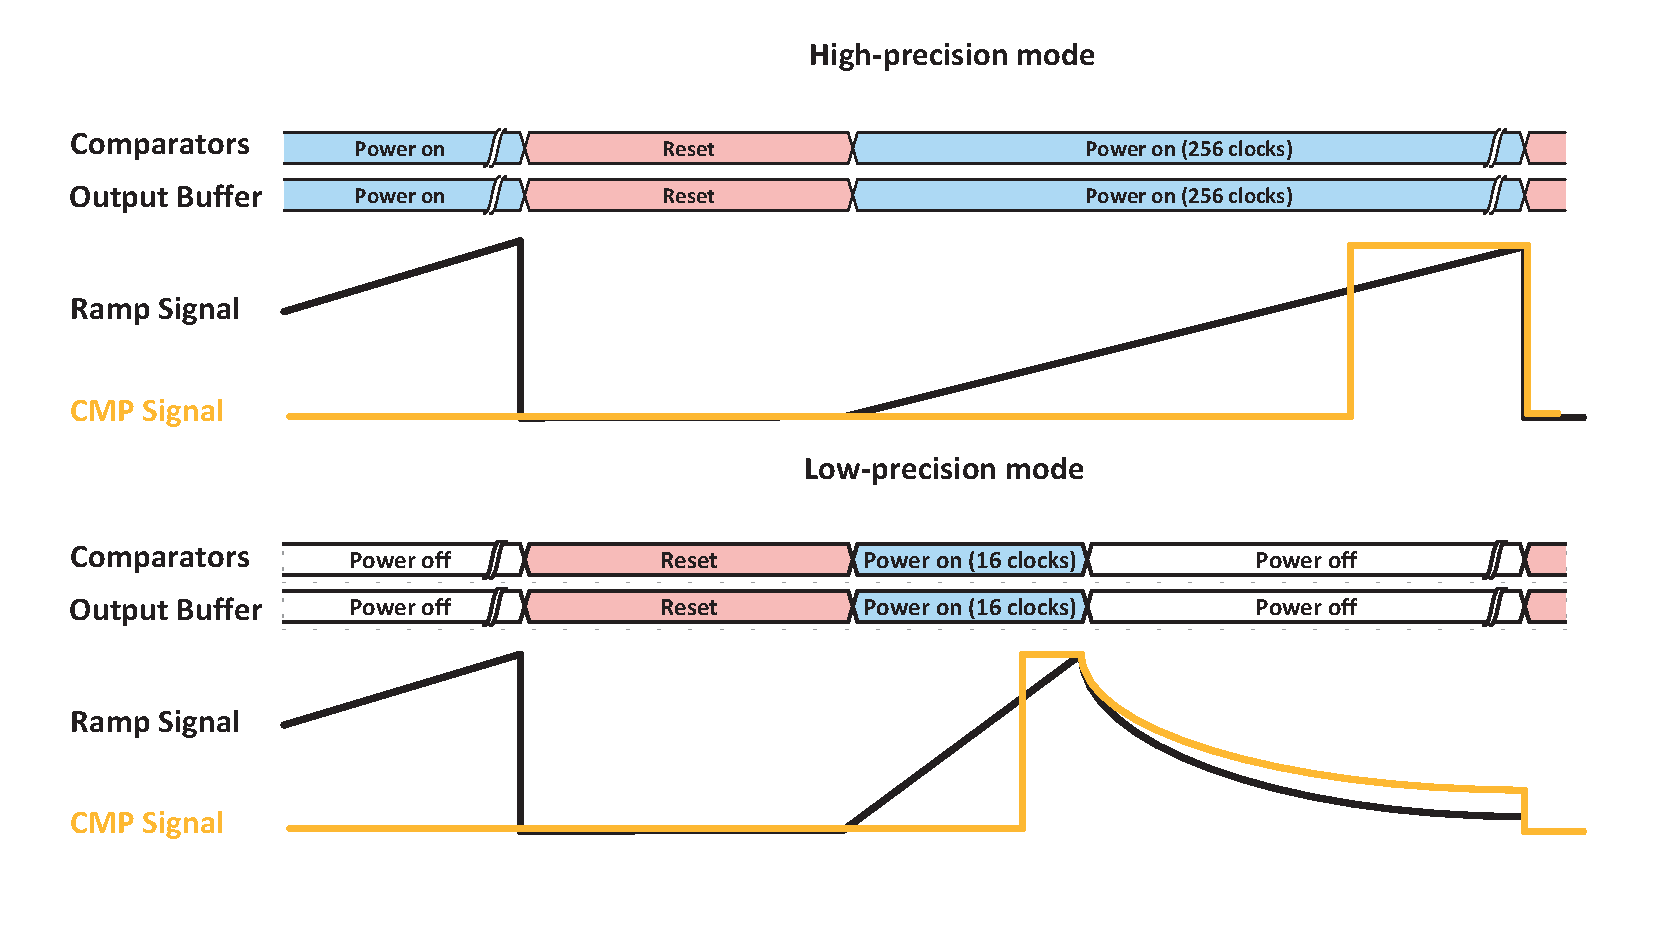
\includegraphics[width=3.5in]{./Figures/SS_pg.eps}}
	\caption{Adaptive-precision and Power Gating Implementation for the SS ADCs.}
	\label{SS_pg}
\end{figure} 

\begin{figure}[htbp]
	\centerline{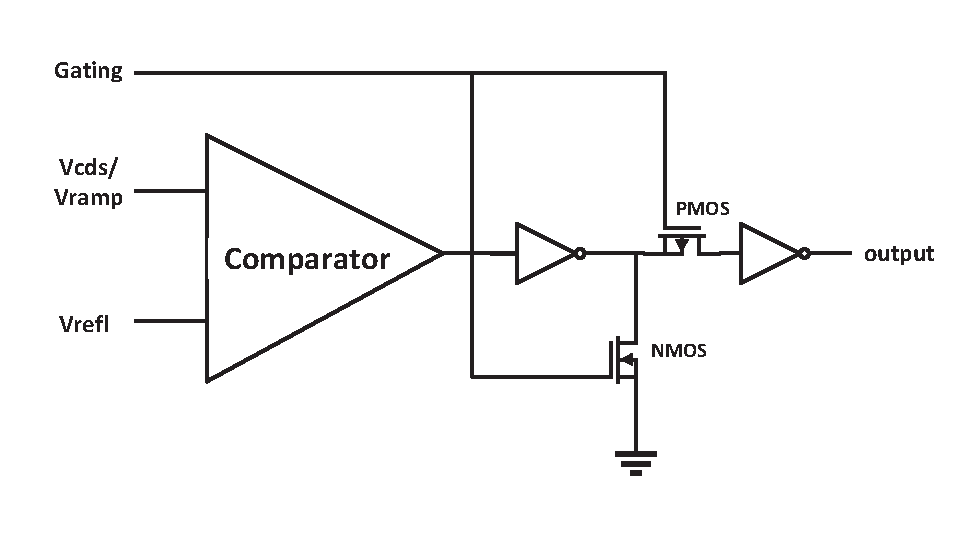
\includegraphics[width=3.5in]{./Figures/MATE.eps}}
	\caption{Two Switches Added to the Inverters Following the Comparator in the SS ADCs.}
	\label{MATE}
\end{figure} 

\subsection{Implementation for the SAR/SS ADCs}

As evaluated in Sect.~\ref{result}, the SAR/SS ADCs’ power consumption is mainly taken up by the column-parallel buffers of reference voltages in the SAR sub-ADCs.
It is because that these buffers need to drive relatively large and changing load capacitance, which means relatively large static and dynamical current is required.
Therefore, gating these buffers will significantly reduce both static power consumption and dynamical power consumption for the ADCs.

In addition, the CDS circuits and comparators in the SAR/SS ADCs also consume a certain amount of energy. However, we only choose to take the comparators under control because they can conveniently share the same gating signal as the buffers'. And the gating signal of the buffers can also be the same as the start signal of the ramp generator. Therefore, gating the buffers and comparators in the SAR/SS ADCs will cost little extra control logic but some shared level-shifters and inverters.

Besides, the power distribution results in Sect.~\ref{result} shows that adaptive-precision tuning is not necessary within the ramp generator of the SAR/SS ADCs, which means the counter in the SAR/SS ADCs do not need to support two modes for adaptive-precision as in the SS ADCs.

The waveform of related signals is presented in Fig.~\ref{SAR_pg}. It is noticed that For low-precison conversion, the ramp signal is generated as usaual but the buffers and comparators will be power off, leaving the 4-bit results converted completely by the SAR logic. 

\begin{figure}[htbp]
	\centerline{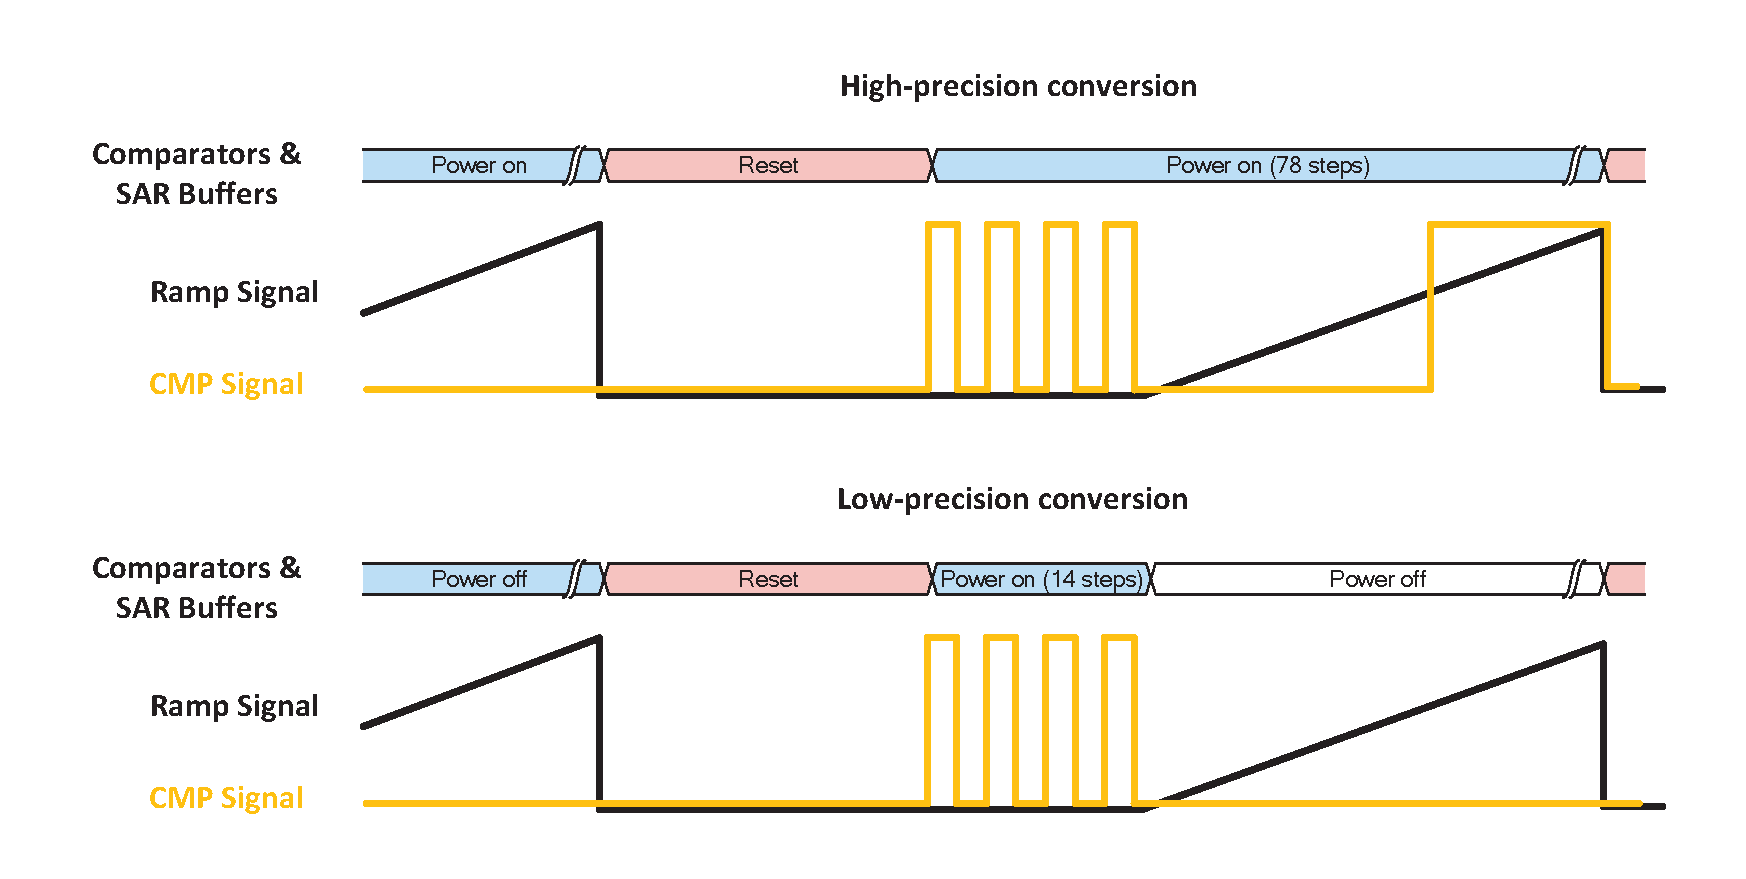
\includegraphics[width=3.5in]{./Figures/SAR_pg.eps}}
	\caption{Adaptive-precision and Power Gating Implementation for the SAR/SS ADCs.}
	\label{SAR_pg}
\end{figure} 
	\section{Evaluation Results}\label{result}

This section presents quantitative evaluation results of the proposed adaptive-precision ADC 
designs, including a column-parallel Single-Slope (SS) ADC and a column-parallel successive 
approximation register (SAR)/SS ADC. Both ADC designs are implemented using TSMC 65nm processing,
and simulated in Virtuoso’s AMS Environment. Circuit power consumption is collectively estimated
based on the average transient current of different ADC modules given one complete sampling and 
conversion period. Power savings are then estimated by comparing the power consumption of the
low-precision conversion mode against that of the high-precision conversion mode. 

Specifically, the detailed power-breakdown and power-saving results of the proposed SS and SAR/SS ADC designs are presented in \ref{SS power} and \ref{SAR power}. And the key design characteristics are summarized in \ref{summary}, with a comparison between our work and previous reported configurable ADCs.

\subsection{Power-scaling Performance of the SS ADC Design}\label{SS power}
%Table~\ref{tab1} summarizes the key design characteristics of the SS ADC design. Considering a 
%$512\times512$ pixel array, the frame rate is 162fps.  The SNDR of the SS ADC is 23.83/46.64 dB, 
%which means the ENOB is 3.67/7.46 bits.  

Fig.~\ref{SSresults1} shows the detailed power-breakdown results of the SS ADC design,
which demonstrates that the power consumption of the SS ADC design is mainly contributed by 
the column-parallel comparators and the output buffer of the ramp generator, both of which 
can be effectively regulated via power gating for low-power conversion. The peripheral circuits include a bandgap and voltage divider, level-shift circuits and global buffers.

The power-saving results are also presented in Fig.~\ref{SSresults2}, where the annotated power consumption is measured and divided by column. It shows that the total power consumption of the low-precision conversion mode is 40.8uW/column, and the power consumption of the high-precision conversion mode is 76.2uW/column. 
Compared to the high-precision conversion mode, the low-precision conversion mode can reduce 
the power consumption approximately 50\%, which is contributed by the power-gating-regulated comparators and buffer.

\iffalse
\begin{table}[htbp]
	\caption{PERFORMANCE OF THE SS ADC DESIGN}
	\begin{center}
		\begin{tabular}{|c|c|}
			\hline
			\textbf{Prameter}& \textbf{Value} \\
			\hhline{|==|}
			\textbf{Process}& 65nm \\
			\hline 
			\textbf{Supply voltage}& 2.5/1.2 V \\
			\hline
			\textbf{Clock Frequency}&	25MHz \\
			\hline
			\textbf{Architecture}&	SS \\
			\hline
			\textbf{Quantization bits}&	4/8 bits\\
			\hline
			\textbf{Conversion time}&	12.04us \\
			\hline
			\textbf{Number of parallel columns}&	512 \\
			\hline
			\textbf{Throughput (samples per second)}&	42.5M \\ 
			\hline
			\textbf{Power (per column)}&	40.8/76.2 uW \\
			\hline
			\textbf{SNDR}& 23.83/46.64 dB@ 8.44 kHz\\
			\hline
			\textbf{ENOB}& 3.67/7.46 bits\\
			\hline
			\textbf{FOM$^{\mathrm{a}}$}& 38.59/5.21 pJ/step\\
			\hline
			\multicolumn{2}{l}{$^{\mathrm{a}}\textbf{FOM}=(\textbf{Power}\ast \textbf{Conversion}\ \textbf{time})/2^{\textbf{ENOB}}$ }	    
		\end{tabular}
		\label{tab1}
	\end{center}
\end{table}
\fi

\begin{figure}[htbp]
	\centerline{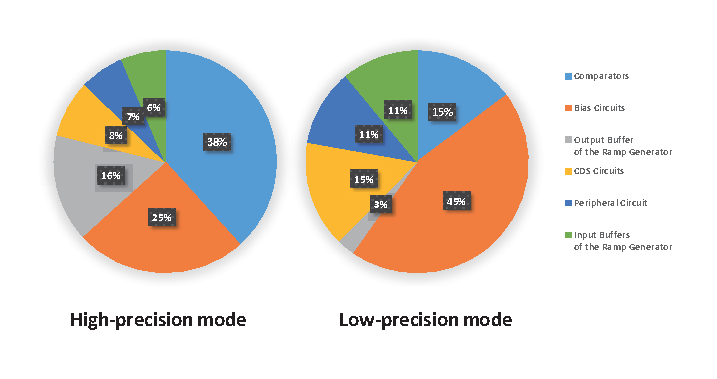
\includegraphics[width=3.5in]{./Figures/SSResults1.eps}}
	\caption{Power-breakdown results of the SS ADC design.}
	\label{SSresults1}
\end{figure}

\begin{figure}[htbp]
	\centerline{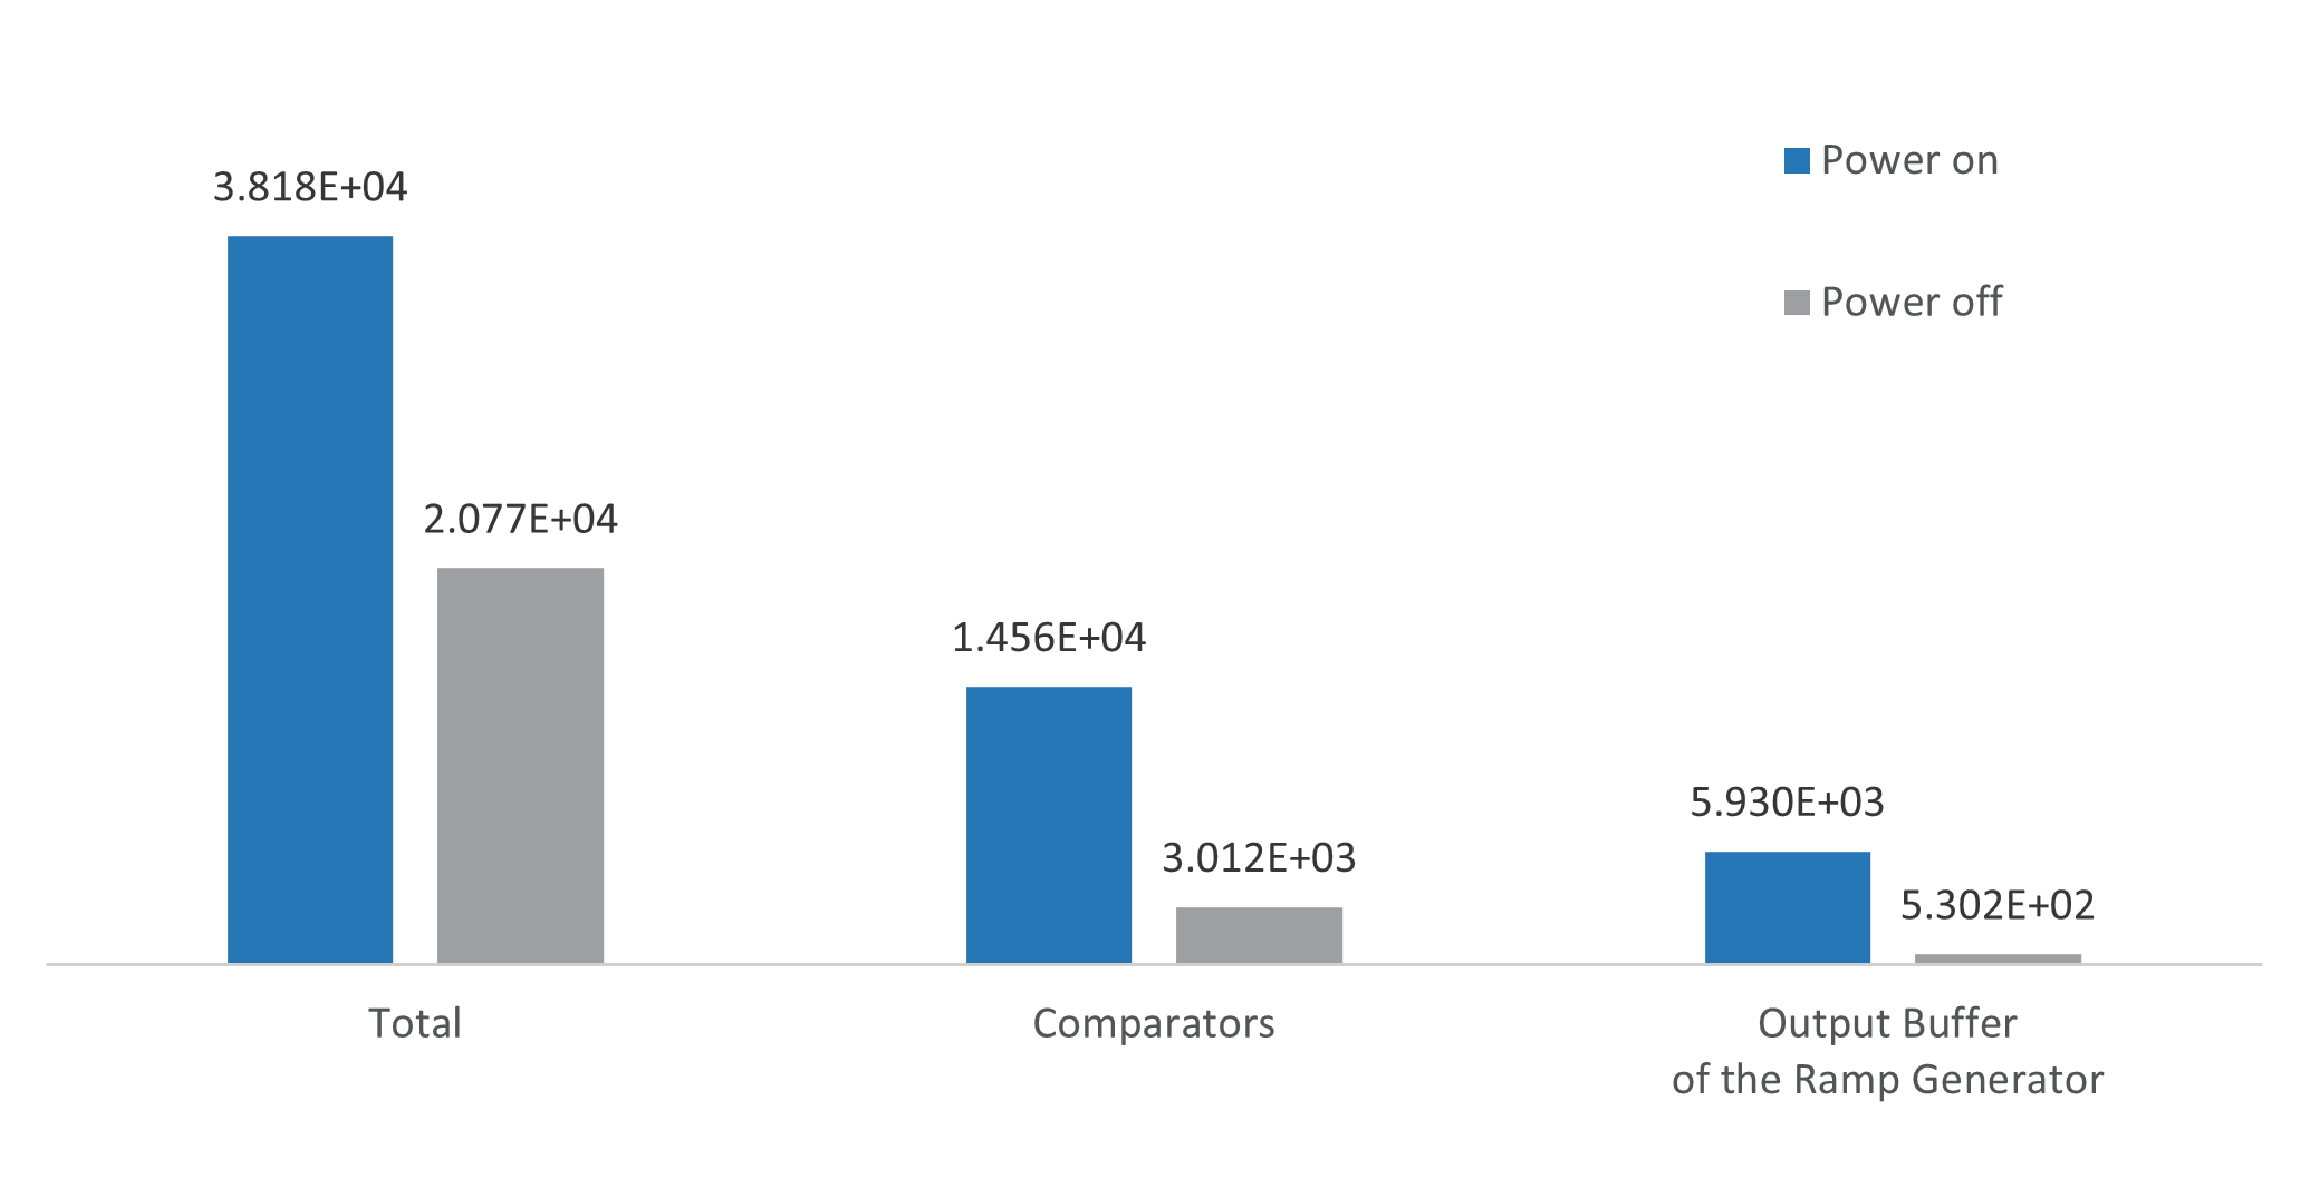
\includegraphics[width=3.5in]{./Figures/SSResults2.eps}}
	\caption{Power-saving results of the SS ADC design.}
	\label{SSresults2}
\end{figure} 

\subsection{Evaluation of the SAR/SS ADC design}\label{SAR power}

%Table~\ref{tab2} summarizes the key design characteristics of the SAR/SS ADC design, for which 
%we consider the same setup as that of the SS ADC. Since fewer steps are required in the SAR/SS ADC 
%design, 1 step is equivalent to 2 clock periods. The SNDR is 24.25/57.87 dB and the ENOB is 3.74/9.32 bits, 
%which is inline with the design specifications. 

Fig.~\ref{SARresults1} shows the detailed power-breakdown results of the SAR/SS ADC design, which 
demonstrates that the power consumption of the SAR/SS ADC design is mainly contributed by the column-parallel buffers of the reference voltages in the sub-ADCs, and power gating can effectively minimize the power consumption of these 
power-dominant components. 

The power-saving results are also presented in Fig.~\ref{SARresults2}, showing that the total power consumption of the SAR/SS ADC design is 256.1uW/column for the high-precision conversion mode and 137.1uW/column for the low-precision conversion mode. 
Compared to the high-precision conversion mode, the low-precision conversion mode can reduce the power consumption approximately 50\%.

\iffalse
\begin{table}[htbp]
	\caption{PERFORMANCE OF THE SAR/SS ADC DESIGN}
	\begin{center}
		\begin{tabular}{|c|c|}
			\hline
			\textbf{Prameter}& \textbf{Value} \\
			\hhline{|==|}
			\textbf{Process}& 65nm \\
			\hline 
			\textbf{Supply voltage}& 2.5/1.2 V \\
			\hline
			\textbf{Clock Frequency}&	20MHz \\
			\hline
			\textbf{Architecture}&	SAR/SS \\
			\hline
			\textbf{Quantization bits}&	4/10 bits \\
			\hline
			\textbf{Conversion time (us)}&	10.1us \\
			\hline
			\textbf{Number of parallel columns}&	512 \\
			\hline
			\textbf{Throughput (samples per second)}&	50.7M \\ 
			\hline
			\textbf{Power (per column)}&	137.1/256.1 uW \\
			\hline
			\textbf{SNDR}& 24.25/57.87 dB@ 10.06 kHz \\
			\hline
			\textbf{ENOB}& 3.74/9.32 bits \\
			\hline
			\textbf{FOM$^{\mathrm{a}}$}& 103.64/4.05 pJ/step\\
			\hline
			\multicolumn{2}{l}{$^{\mathrm{a}}\textbf{FOM}=(\textbf{Power}\ast \textbf{Conversion}\ \textbf{time})/2^{\textbf{ENOB}}$ }	    
		\end{tabular}
		\label{tab2}
	\end{center}
\end{table}
\fi

\begin{figure}[htbp]
	\centerline{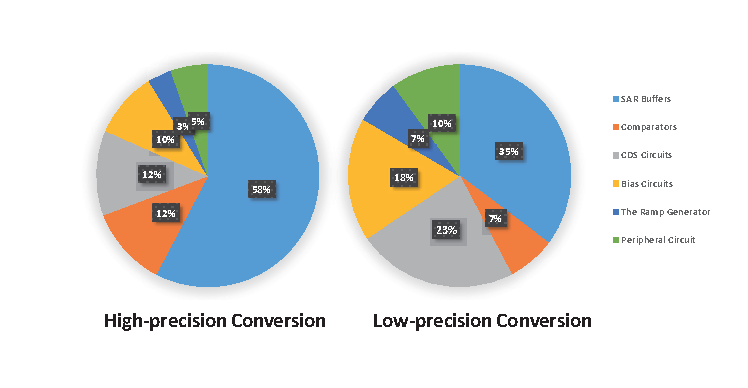
\includegraphics[width=3.5in]{./Figures/SARResults1.eps}}
	\caption{Power-breakdown results of the SAR/SS ADC design.}
	\label{SARresults1}
\end{figure} 

\begin{figure}[htbp]
	\centerline{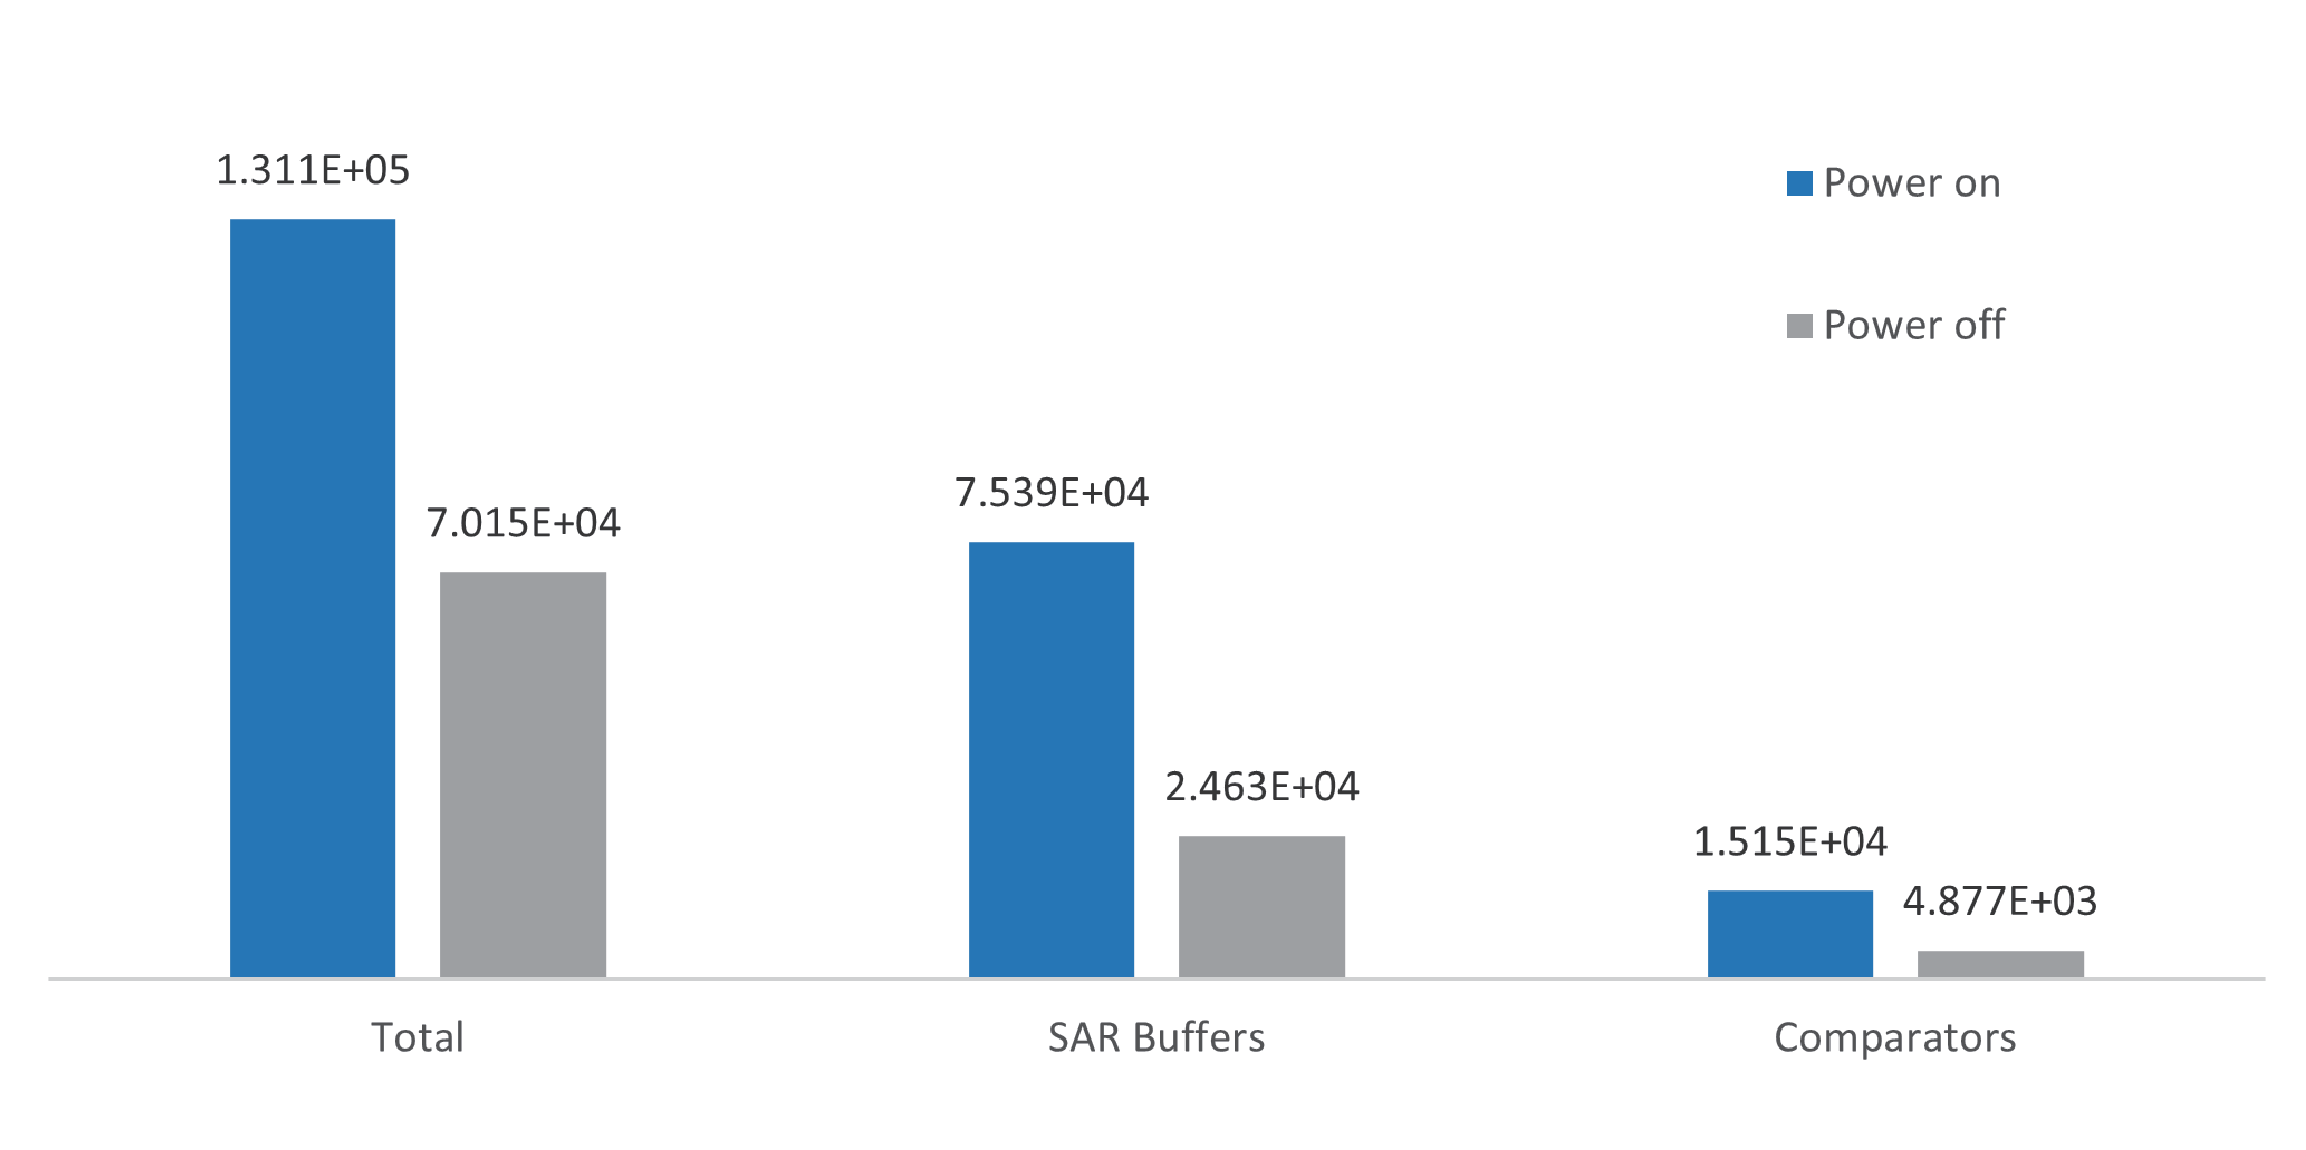
\includegraphics[width=3.5in]{./Figures/SARResults2.eps}}
	\caption{Power-saving results of the SAR/SS ADC design.}
	\label{SARresults2}
\end{figure} 

\subsection{Performance Summary and Comparison}\label{summary}

Table~\ref{tab1} summarizes the key characteristics of the proposed SS and SAR/SS ADC designs.
And a comparison with previous reported configurable ADCs is also provided. 
We take the precision-adaptive SAR ADCs into comparison because on the one hand they have similar precision and sampling rate configurations to our design, on the other hand, SAR ADCs are also applicable to column-parallel image processing given a relatively loose area constraint.

It is highlighted that our design achieves better power-scaling performance than previous works. And the presented power-scaling percents of the SAR ADCs can actually be worse because in these works only the power consumption of the core ADC circuit is measured, while we have analysed the power consumption of the whole implementation, including the bandgap, voltage divider, bias circuits and reference buffers. Therefore, with fair considerations of the peripheral fixed parts of energy, the power-scaling performance of our design can definitely be more competitive.

It is noted that the overall power consumption of the proposed implementation is relatively high. However, since the design studies are targeting to exploit the power-scaling capabilities with applying reasonable power gating strategies, rather than shrinking the power consumption as more as possible for the ADCs equipped with fixed-precision, instructive power-saving performance is still effectively demonstrated.

\begin{table*}[htbp]
	\caption{PERFORMANCE AND COMPARISON}
	\begin{center}
		\begin{tabular}{|c|c|c|c|c|c|c|c|c|}
			\hline
			\textbf{}& \multicolumn{2}{|c|}{\cite{zhu_6--10-bit_2015}} & \multicolumn{2}{|c|}{\cite{zhu_6--10-bit_2015}} & \multicolumn{4}{|c|}{This work} \\
			\hhline{|=========|}
			%\iffalse
			\textbf{Process}& \multicolumn{2}{|c|}{180nm} & \multicolumn{2}{|c|}{65nm} & \multicolumn{4}{|c|}{65nm} \\
			\hline 
			\textbf{Supply voltage}& \multicolumn{2}{|c|}{0.6V} & \multicolumn{2}{|c|}{0.4V-1V} & \multicolumn{4}{|c|}{2.5V(Analog), 1.2V(Digital)} \\
			\hline
			
			%\textbf{Clock Frequency}&	20MHz \\
			%\hline
			\textbf{Architecture}& \multicolumn{2}{|c|}{SAR} & \multicolumn{2}{|c|}{SAR} & \multicolumn{2}{|c|}{SS} & \multicolumn{2}{|c|}{SAR/SS}\\
			\hline
			\textbf{Precison(bits)} & 8 & 10 & 8 & 10 & 4 & 8 & 4 & 10 \\
			\hline
			\textbf{Sampling rate(Hz)}& \multicolumn{2}{|c|}{100K} & \multicolumn{2}{|c|}{20K} & \multicolumn{2}{|c|}{83K} & \multicolumn{2}{|c|}{99K} \\
			\hline
			%\textbf{Number of parallel columns}&	512 \\
			%\hline
			%\textbf{Throughput (samples per second)}&	50.7M \\ 
			%\hline
			\textbf{SNDR(dB)} & 47.4 & 60.5 & 47.0 & 55.0 & 23.83 & 46.64 & 24.25 & 57.87 \\
			\hline
			\textbf{ENOB(bits)}& 7.58 & 9.76 & 7.51 & 8.84 & 3.67 & 7.46 & 3.74 & 9.32 \\
			\hline
			\textbf{Power consumption}& 0.32$\mu$W & 0.52$\mu$W &  0.146$\mu$W & 0.206$\mu$W & 40.8$\mu$W & 76.2$\mu$W & 137.1$\mu$W & 256.1$\mu$W\\
			\hline
			\textbf{Power-scaling performance}& 62\% & 100\% & 71\% & 100\% & \textbf{54}\% & 100\% & \textbf{54}\% & 100\% \\
			\hline
			%\fi
			%\textbf{FOM$^{\mathrm{a}}$}& 103.64/4.05 pJ/step\\
			%\hline
			%\multicolumn{2}{l}{$^{\mathrm{a}}\textbf{FOM}=(\textbf{Power}\ast \textbf{Conversion}\ \textbf{time})/2^{\textbf{ENOB}}$ }	    
		\end{tabular}
		\label{tab1}
	\end{center}
\end{table*}
	\section{Discussions}\label{discussion}
Combining adaptive-precision with fine-grained power gating strategies, both the SS ADCs and SAR/SS ADCs can save energy dynamically and significantly with only a few required control circuits. 
It is because that in the column-parallel and SS-logic-adopted ADCs, not only a large amount of currents can be under control but also the power gated time can be continously long. 

In comparison, the SAR/SS ADCs can support higher quantization bits and require fewer extra control circuits for the adaptive-precision, 
while SS ADCs inherently require less area and can be applied to the 4/8-bit situation more effectively. 
Therefore, according to specific design specifications, different structures can be chosen. 

For other different precision configurations and number of parallel collumns, 
the corresponding power consumption and energy-saving performance can also be estimated with extending the evaluation results in Sect.~\ref{result}.
	\section{Conclusions}\label{conclusion}

This article introduces an adaptive-precision ADC architecture to enable energy-efficient 
data analysis pipeline for edge computing. Two adaptive-precision ADC designs are implemented, 
including a column-parallel single-slope (SS) ADC and a column-parallel successive approximation 
register (SAR)/SS ADC. The proposed method is efficient and easy to implement. Experimental results 
demonstrate that the proposed adaptive-precision method can improve the ADC power efficiency by 
approximately 50\%. Future work will consider applying the proposed method to other ADC architectures, 
as well as system integration with deep-learning computing engine to enable adaptive-precision
data analysis pipeline for energy efficient edge intelligence. 

%According to the evaluation results of two CIS-applied column-parallel ADC designs, almost a half of the ADCs’ power consumption can be reduced for low-precision conversion by power gating, while only a few of extra control circuits is required.  It is because that in column-parallel ADCs where the SS conversion logic is widely adopted, not only can large amounts of current be under control but also the power gating time can be continuously and exponentially scalable.  As the proposed architecture may resonate with varying downstream deep-learning algorithms for efficient multi-tasks analysis, further works on the co-design of ADCs and algorithms remain to be developed for more intelligent edge computing.

	
	\bibliographystyle{IEEEtran}
	\bibliography{main}
	
\end{document}